\documentclass[12pt, oneside]{book}\usepackage{knitr}

%%%%%%%%%%%%%%%%%%%%%%%%%%%%%%%%%%%%%%
% packages
%%%%%%%%%%%%%%%%%%%%%%%%%%%%%%%%%%%%%%
\usepackage[margin=1in]{geometry}
\usepackage[T1]{fontenc}
\usepackage{amsmath,dsfont}
\usepackage{caption}
\usepackage{floatrow}
% \usepackage[maxbibnames=99, backend=biber, giveninits=true, natbib=true, uniquename=init, style=apa]{biblatex}
% \DeclareLanguageMapping{english}{english-apa}

%\renewcommand{\baselinestretch}{1.5} % line spacing (for the journal) 
\usepackage[utf8]{inputenc}
\usepackage{bm}
\usepackage{verbatim}
\usepackage{float}
\usepackage{mwe}
\usepackage{color,soul}
\usepackage{threeparttable}
\usepackage{graphicx}
\usepackage{subcaption}
\usepackage{mwe}
\usepackage{mdframed}
\usepackage{xcolor}
\usepackage{bbm}
%\usepackage{authblk}

\usepackage{hyperref}
% References
\usepackage[
backend=bibtex,
style=authoryear,
sorting=ynt,
natbib=true
]{biblatex}
% \renewcommand{\citet}[#1]{\textcite{#1}}
%\usepackage{natbib}
%\bibliographystyle{apalike}
%\bibpunct[, ]{(}{)}{,}{a}{}{,}%
%\def\bibfont{\small}%
%\def\bibsep{\smallskipamount}%
%\def\bibhang{24pt}%
%\def\newblock{\ }%
%\def\BIBand{and}%

%\soulregister\cite7
%\soulregister\ref7
%\soulregister\eqref7
%\soulregister\pageref7
%\soulregister\equation7

\usepackage{multirow}
\usepackage{makecell}
\usepackage{booktabs}
\usepackage{array}
\usepackage{hhline}
\renewcommand\theadalign{bc}
\renewcommand\theadfont{\bfseries}
\renewcommand\theadgape{\Gape[4pt]}
\renewcommand\cellgape{\Gape[4pt]}
\usepackage{lscape}
\usepackage{mathtools}
\usepackage{bbm}
\usepackage{romanbar}
\usepackage{amsthm}
\usepackage{enumerate}
\usepackage{rotating}
\usepackage{tikz}
\usetikzlibrary{matrix}
\usetikzlibrary{calc,intersections}
\usepackage{mathrsfs}

%%%%
\usepackage{color}
\newcommand{\colr}[1]{{\color{red} {#1}}}
\newcommand{\colb}[1]{{\color{blue} {#1}}}
%%%%%%%%%%%%%%%%%%%%%%%%%%%%%%%%%%%%%%
% definitions
%%%%%%%%%%%%%%%%%%%%%%%%%%%%%%%%%%%%%%
\newtheorem{theorem}{Theorem}[section]
\newtheorem{corollary}[theorem]{Corollary}
\newtheorem{lemma}[theorem]{Lemma}
\newtheorem{proposition}[theorem]{Proposition}

% Definitions  etc.
\theoremstyle{definition}
\newtheorem{definition}[theorem]{Definition}
\newtheorem{example}{Example}[section]
\theoremstyle{remark}
\newtheorem{remark}[theorem]{Remark}
\newtheorem{observation}[theorem]{Observation}

%%%%%%%%%%%%%%%%%%%%%%%%%%%%%%%%%%%%%%
% Math commands
%%%%%%%%%%%%%%%%%%%%%%%%%%%%%%%%%%%%%%
\newcommand{\bol}[1]{\mbox{\boldmath$#1$}}
\newcommand{\mb}[1]{\mathbf{#1}}
\newcommand{\eqdist}{\stackrel{d}{=}}
\newcommand{\bSigma}{\mathbf{\Sigma}}
\newcommand{\hbSigma}{\hat{\bol{\Sigma}}}
\newcommand{\bDelta}{\bol{\Delta}}
\newcommand{\hw}{\hat{w}}
\newcommand{\bmu}{\bol{\mu}}
\newcommand{\hbmu}{\hat{\bol{\mu}}}
\newcommand{\tbmu}{\tilde{\bol{\mu}}}
\newcommand{\bet}{\bol{\eta}}
\newcommand{\btheta}{\bol{\theta}}
\newcommand{\bb}{\mathbf{b}}
\newcommand{\hbb}{\mathbf{\hat{b}}}
\newcommand{\bx}{\mathbf{x}}
\newcommand{\bxb}{\bar{\mathbf{x}}}
\newcommand{\bQ}{\mathbf{Q}}
\newcommand{\hbQ}{\hat{\mathbf{Q}}}
\newcommand{\be}{\mathbf{e}}
\newcommand{\by}{\mathbf{y}}
\newcommand{\byb}{\bar{\mathbf{y}}}
\newcommand{\tby}{\tilde{\mathbf{y}}}
\newcommand{\bt}{\mathbf{t}}
\newcommand{\bC}{\mathbf{C}}
\newcommand{\bP}{\mathbf{P}}
\newcommand{\bM}{\mathbf{M}}
\newcommand{\bH}{\mathbf{H}}
\newcommand{\bL}{\mathbf{L}}
\newcommand{\bl}{\mathbf{l}}
\newcommand{\br}{\mathbf{r}}
\newcommand{\hbm}{\bol{\hat{\mu}}}
\newcommand{\hbet}{\bol{\hat{\eta}}}
\newcommand{\bhR}{\hat{\mathbf{R}}}
\newcommand{\bhA}{\hat{\mathbf{A}}^{-1}}
\newcommand{\bR}{\mathbf{R}}
\newcommand{\btR}{\mathbf{\tilde{R}}}
\newcommand{\bz}{\mathbf{z}}
\newcommand{\bd}{\mathbf{d}}
\newcommand{\bB}{\mathbf{B}}
\newcommand{\bE}{\mathbf{E}}
\newcommand{\bX}{\mathbf{X}}
\newcommand{\bY}{\mathbf{Y}}
\newcommand{\bv}{\mathbf{v}}
\newcommand{\bw}{\mathbf{w}}
\newcommand{\hbw}{\mathbf{\hat{w}}}
\newcommand{\btL}{\mathbf{\tilde{L}}}
\newcommand{\bOne}{\mathbf{1}}
\newcommand{\bzero}{\mathbf{0}}
\newcommand{\bI}{\mathbf{I}}
\newcommand{\xp}{\mbox{exp}}
\newcommand{\tr}{\operatorname{tr}}
\newcommand{\Cov}{\mbox{Cov}}
\newcommand{\E}{\mbox{E}}
\newcommand{\Var}{\mbox{Var}}
\newcommand{\ve}{\mbox{vec}}
\newcommand{\tbx}{\tilde{\bx}}
\newcommand{\bA}{\bol{A}}
\newcommand{\ba}{\bol{a}}
\newcommand{\brx}{\breve{\bx}}
\newcommand{\brm}{\breve{\bol{\mu}}}
\newcommand{\brA}{\breve{\bA}}
\newcommand{\si}{\boldsymbol{\sigma}}
\newcommand{\tbF}{\tilde{\mathbf{\Phi}}}
\newcommand{\bF}{\mathbf{F}}
\newcommand{\bn}{\boldsymbol{\nu}}
\newcommand{\byy}{\bn_y}
\newcommand{\bxi}{\boldsymbol{\xi}}
\newcommand{\bD}{\mathbf{D}}
\newcommand{\eps}{\pmb{\varepsilon}}
\newcommand{\bW}{\mathbf{W}}
\newcommand{\bV}{\mathbf{V}}
\newcommand{\bla}{\boldsymbol{\lambda}}
\newcommand{\bry}{\breve{\by}}
\newcommand{\tbw}{\tilde{\bw}}
\newcommand{\tbSigma}{\tilde{\bSigma}}
\newcommand{\bO}{\mathbf{O}}
\newcommand{\brn}{\breve{\bn}}
\newcommand{\bOmega}{\boldsymbol{\Omega}}
\newcommand{\bomega}{\boldsymbol{\omega}}
\newcommand{\tbn}{\tilde{\bn}}
\newcommand{\tbB}{\tilde{\bB}}
\newcommand{\tbb}{\tilde{\mathbf{b}}}
\newcommand{\bS}{\mathbf{S}}
\newcommand{\sx}{\bar{\mathbf{x}}}
\newcommand{\sy}{\bar{\mathbf{y}}}
\newcommand{\Tr}{\text{tr}}
\newcommand{\bG}{\mathbf{G}}
\newcommand{\bu}{\mathbf{u}}
\newcommand{\bU}{\mathbf{U}}
\newcommand{\bTheta}{\mathbf{\Theta}}
\newcommand{\ta}{\alpha}
\newcommand{\tb}{\beta}
\newcommand{\bZ}{\mathbf{Z}}
\newcommand{\bT}{\mathbf{T}}
\newcommand{\bq}{\mathbf{q}}
% \newcommand{\bt}{\mathbf{t}}
\newcommand{\hbtheta}{\bol{\hat{\theta}}}
\newcommand{\ones}{\mathbf{1} }
\newcommand{\bgamma}{ \boldsymbol{\gamma} }
\newcommand{\bGamma}{ \boldsymbol{\Gamma} }
\newcommand{\optn}[1]{\operatorname{#1}}
\newcommand{\VaR}{\operatorname{VaR}}
\newcommand{\CVaR}{\operatorname{CVaR}}
\newcommand{\prob}{\mathsf{P}}
\newcommand{\real}{\mathbb{R}}
\newcommand{\Kappa}{\mathrm{K}}
\newcommand{\argmin}{\mathop{\mathrm{argmin}}}

% Portfolio characteristics
\newcommand{\hV}{\hat{V}_{GMV}}
\newcommand{\hR}{\hat{R}_{GMV}}
\newcommand{\R}{R_{GMV}}
\newcommand{\V}{V_{GMV}}
\newcommand{\hs}{\hat{s}}

\providecommand{\keywords}[1]
{
\small	
\textbf{\textit{Keywords}:} #1
}

\renewcommand \thesubsubsection{\roman{subsubsection}.\roman{subsubsection}}


\DeclareNewFloatType{chunk}{placement=H, fileext=chk, name=}
\captionsetup{options=chunk}
\renewcommand{\thechunk}{Chunk~\thesection.\arabic{chunk}}
\makeatletter
\@addtoreset{chunk}{section}
\makeatother
\makeatletter

\title{Optimal portfolios -- estimation and uncertainty assessment in the high-dimensional setting}
\author{Erik Thorsén}
\date{}

\newcommand{\email}{erik.thorsen$@$math.su.se}
\newcommand{\auth}{Erik Thorsén}
\newcommand{\yr}{2022}
\newcommand{\address}{Matematiska Institutionen, Stockholms Universitet, 106 91 Stockholm}

\addbibresource{references.bib}
\addbibresource{references-thesis.bib}
\IfFileExists{upquote.sty}{\usepackage{upquote}}{}
\begin{document}




%%%%%% ------------------------------------------------------------------------
%%%%%% FRONTMATTER
%%%%%% ------------------------------------------------------------------------
\frontmatterSU

\maketitle

%: ----------------------- Cover page back side ------------------------

\newpage

%Financial portfolios and diversification go hand in hand.
Diversification is one of, if not, the best risk mitigation strategy there is.
If an investment performs poorly, then it will not impact the performance of the portfolio much due to diversification.
Modern Portfolio Theory (MPT) is a framework for constructing diversified portfolios.
However, MPT relies on unknown parameters that need to be estimated.
By using estimates, estimation uncertainty is introduced to the allocation problem.
This thesis contains five papers which provide results on how to deal with estimation uncertainty in very large sample portfolios from the MPT framework.
These results provide tools to better understand the investment process and the empirical results that can be observed.

Paper 1 explores all of the portfolios that can be placed in the framework of MPT. 
The paper provides the sampling distribution for all optimal portfolios and their characteristics.
This is done by assuming that the returns follow a multivariate normal distribution.
Furthermore, the high-dimensional asymptotic joint distribution for the quantities of interest is derived.
A simulation study shows that the high-dimensional distribution can provide a good approximation to the finite sample one.

Paper 2 continues on the idea of paper 1.
It considers the quadratic utility allocation problem from paper 1 with an additional risk-free asset in the portfolio.
The portfolio is usually known as the Tangency Portfolio (TP).
The distribution of the sample TP weights is derived under a skew-normal distribution.
Results show that skewness implies a bias in the finite sample TP weights.
The bias dissapears in the high-dimensional distribution.

Paper 3 takes on a practical aspect of investing, namely how to transition from one portfolio to another.
A reallocation scheme is developed, which minimizes the out-of-sample variance of the Global Minimum Variance (GMV) portfolio, given a holding portfolio. 
The holding portfolio is the portfolio which the investor currently owns.
An extensive simulation study show that the reallocation scheme can provide accurate estimates of the portfolio variance.
Furthermore, an empirical application shows that the scheme provides the smallest out-of-sample variance in comparison to a number of benchmarks.
The theoretical results from this paper are implemented in the DOSPortfolio R-package.

Paper 4 derives properties of two different performance measures for three different high-dimensional GMV portfolio estimators. 
The measures are the out-of-sample variance and loss.
The former is always used as an evaluation metric in empirical applications.
The results show that the latter metric, the out-of-sample loss, does not need the same stringent assumptions as the out-of-sample variance in the high-dimensional setting.
Using the out-of-sample loss, the performance of the three different portfolios can be ordered.
This order is verified in a simulation study and an empirical application.

Paper 5 extends the results of papers 3 and 4. 
It introduces Thikonov regularization to the GMV portfolio weights as well as linear shrinkage.
A simulation study shows that the method is preferable to a number of benchmarks. 
Furthermore, an empirical application shows that it can provide the smallest out-of-sample variance and provide good characteristics for the portfolio weights. % Uncomment to input the abstract if you want to have it printed.

\phantom{.}

\vspace{\stretch{1}}

{\fontfamily{\familydefault}\selectfont
{\scriptsize
\noindent
\copyright \auth, Stockholm, \yr % Name of author, location year
\newline
Address: \address
\newline
E-mail address: \email
 
\vspace{5mm}
\noindent
ISBN XXX-XX-XXXX-XXX-X % Provided by the library: disputationer@su.se

\vspace{5mm}
\noindent
Printed in Sweden by Printing Company, Stockholm, \yr %name of printing company

\noindent
Distributor: Department of Mathematics, Stockholm University %name of department
}
}
\cleardoublepage

% to remove 
% \chapter*{\centering Abstract}
% Financial portfolios and diversification go hand in hand.
Diversification is one of, if not, the best risk mitigation strategy there is.
If an investment performs poorly, then it will not impact the performance of the portfolio much due to diversification.
Modern Portfolio Theory (MPT) is a framework for constructing diversified portfolios.
However, MPT relies on unknown parameters that need to be estimated.
By using estimates, estimation uncertainty is introduced to the allocation problem.
This thesis contains five papers which provide results on how to deal with estimation uncertainty in very large sample portfolios from the MPT framework.
These results provide tools to better understand the investment process and the empirical results that can be observed.

Paper 1 explores all of the portfolios that can be placed in the framework of MPT. 
The paper provides the sampling distribution for all optimal portfolios and their characteristics.
This is done by assuming that the returns follow a multivariate normal distribution.
Furthermore, the high-dimensional asymptotic joint distribution for the quantities of interest is derived.
A simulation study shows that the high-dimensional distribution can provide a good approximation to the finite sample one.

Paper 2 continues on the idea of paper 1.
It considers the quadratic utility allocation problem from paper 1 with an additional risk-free asset in the portfolio.
The portfolio is usually known as the Tangency Portfolio (TP).
The distribution of the sample TP weights is derived under a skew-normal distribution.
Results show that skewness implies a bias in the finite sample TP weights.
The bias dissapears in the high-dimensional distribution.

Paper 3 takes on a practical aspect of investing, namely how to transition from one portfolio to another.
A reallocation scheme is developed, which minimizes the out-of-sample variance of the Global Minimum Variance (GMV) portfolio, given a holding portfolio. 
The holding portfolio is the portfolio which the investor currently owns.
An extensive simulation study show that the reallocation scheme can provide accurate estimates of the portfolio variance.
Furthermore, an empirical application shows that the scheme provides the smallest out-of-sample variance in comparison to a number of benchmarks.
The theoretical results from this paper are implemented in the DOSPortfolio R-package.

Paper 4 derives properties of two different performance measures for three different high-dimensional GMV portfolio estimators. 
The measures are the out-of-sample variance and loss.
The former is always used as an evaluation metric in empirical applications.
The results show that the latter metric, the out-of-sample loss, does not need the same stringent assumptions as the out-of-sample variance in the high-dimensional setting.
Using the out-of-sample loss, the performance of the three different portfolios can be ordered.
This order is verified in a simulation study and an empirical application.

Paper 5 extends the results of papers 3 and 4. 
It introduces Thikonov regularization to the GMV portfolio weights as well as linear shrinkage.
A simulation study shows that the method is preferable to a number of benchmarks. 
Furthermore, an empirical application shows that it can provide the smallest out-of-sample variance and provide good characteristics for the portfolio weights.

\begin{dedication}
{\fontfamily{calligra}\selectfont
{\Large
Till min familj.
}
}
\end{dedication}
%%%%%

\chapter*{List of papers}
\nocite{bodnar2019sampling_thesis, javed2021tangency_thesis, bodnar2021dynamic_thesis, bodnar2021empirical_thesis, bodnar2022double_thesis, bodnar2021quantile_thesis, bodnar2020quantile_thesis, bodnar2021bayesian_thesis, DOSPortfolio_thesis}
The following section include the results produced in the writing of this thesis.

\printbibliography[keyword={included_in_thesis}, title={Papers included in this thesis}, heading=subbibliography]

\textbf{Author contribution:} 
E. Thors\'en has actively contributed to developing the content of all papers.
In the first paper, E. Thors\'en contributed with the derivation of the theoretical results and with writing the majority of the paper in collaboration with all other authors. The original idea was presented by T. Bodnar.
In the second paper, E. Thors\'en contributed with the theoretical derivations and writing the majority of the paper in collaboration of S. Mazur and F. Javed. The original idea was presented by S. Mazur and F. Javed.
The original idea of the third paper was born from discussions with T. Bodnar and N. Parolya. 
In this paper, E. Thors\'en contributed with the theoretical derivations and the writing of the paper.
The original idea of the fourth paper stemmed from discussions from the third paper together with T. Bodnar and N. Parolya.
In this paper, E. Thors\'en contributed with the theoretical derivations and the writing of the paper.
The fifth paper also sprung from the third and fourth paper. 
In this paper, E. Thors\'en contributed to the theoretical derivations, the writing of the paper and the idea behind it.
E. Thorsén carried out all computer implementations in all articles.
In all other aspects the authors contributed equally.

\textbf{General comment:} An earlier version of \citet{bodnar2020sampling_thesis} was included in the Licenciate thesis of E. Thors\'en, \citet{thorsen2019assessment}.

\printbibliography[keyword={papers_list}, heading=subsubbibliography]


\chapter*{Acknowledgements}
Early in my graduate studies I asked a professor what it takes to complete a PhD and he answered grit.
The purpose of a PhD is to spend a number of years intensively digging deeper into a subject, coming up with ideas that most often have been solved, does not seem to be solvable or cannot be solved at all.
It is a very humbling experience and there are many people that I would like to thank for making it a fun one as well!

The first person to thank is my supervisor Taras Bodnar.
I am immensely grateful for your guidance, knowledge and discussions over the years.
Thank you for giving me the opportunity of doing this.
I could not have asked for a better supervisor.
I also want to thank my co-supervisor Joanna Tyrcha for your support.

I want to give special thanks to my co-authors that also made this an exciting and great learning experience.
Nestor Parolya, whom I have gotten the pleasure to work extensively with over the last few years. 
You are a co-author of almost all the papers in this thesis and it has been a joy.
I have learned a lot from our discussions.
Thank you, Stepan Mazur and Farrukh Javed for the fun discussions and great collaborations!
Furthermore, thank you Vilhelm Niklasson, Mathias Lindholm and Holger Dette for the (very) long and rewarding discussions! 

Thank you Ola Hössjer for letting me be a part in developing and teaching the course Statistical Data Processing.
I have learned so much from the experience and grown as a person from it!

I also want to thank all my colleagues at the Department of Mathematics.
It has been a incredibly fun place to work and I think that the environment has been, and will continue to be, great.
There are a number of individuals that have made my experience even better.
Thank you Vilhelm, Gustav and Stanislas for being wonderful people to share an office with.
I hope to continue our brewing adventures Vilhelm and the wonderful banter Gustav!
I also want to thank Felix, Måns, Sebastian and Hampus whom I have gotten to spend a lot of time with during the COVID-19 pandemic. 
It made everything so much easier.

Last but not least, I cannot express enough love and gratitude towards my family. 
Mom, dad and my beloved sister, I cannot thank you enough for all your support.
Johanna, you make me a much happier person and I look forward to many more years with you and our son Gabriel. 

\newpage

\tableofcontents
%%%%%% ------------------------------------------------------------------------
%%%%%% END OF FRONTMATTER
%%%%%% ------------------------------------------------------------------------
\mainmatterSU

\part{Introduction}
%%%%%% ------------------------------------------------------------------------
\chapter{Decisions, uncertainty and asset allocations}\label{ch:intro}
%%%%%% ------------------------------------------------------------------------
% General introduction to why portfolio theory and allocations are hard
% ca 1page
A portfolio is a combination of assets.
An asset might be a house, a stock, the value of a contract or any object with a price that can potentially be bought or sold.
The price of an asset develops over time.
The house prices in Stockholm, Sweden, have increased a lot in the past years\footnote{\url{https://www.maklarstatistik.se/omrade/riket/stockholms-lan/\#/villor/48m-prisutveckling}}.
However, the future price for a house is uncertain, especially given that house prices are close to all-time highs.
Will the price continue to increase or will it decrease?
If there is a change, how big will it be?
Depending on the answer, one strategy might be to sell the house today, rent something instead and buy a new house when prices have decreased.
However, to make a decision on whether or not the house should be sold today, there is a need to specify its future value. 
The future is unknown or random, in some sense.
There are many possible changes in the assets value, both in direction and magnitude.
In the context of a model there is a possibility to predict the future price through the use of historical prices.
The decision process now includes even more uncertainty.
There is uncertainty from the choice of model, the perception of past and future prices, and the uncertainty from using estimates instead of the ''true'' parameters for the model.
If the house is one asset among many then there can be as many sources of uncertainty as there are assets, if not more.
The allocation itself, in this case selling the house, is uncertain.
Uncertainty is everywhere in decisions.

The market price of a house is rarely observed.
As a matter of fact, it is only observed when it is sold.
Even though prices are rarely observed there might be houses that are similar.
There are many measurements from the same population, in this case houses which are similar to the one being sold. 
This might not be the case for the second asset that is listed above, a stock.
The frequency of which the price of a stock is observed can be much higher.
On the other hand, there is only one stock with one accompanying time series.
This makes the analysis slightly different.
There can be a lot of historical data, but no identical copies of the stock that can be used to compare and extract information from.
Prices can only be observed as they develop.

In this thesis, the aim is not to predict tomorrows price of an asset but to answer what amount of a budget should be spent on the different assets in the long run.
The methods in this thesis build upon the seminal work of \citet{markowitz1959portfolio}, what is known as Modern Portfolio Theory (MPT).
Markowitz argued that any portfolio which simply maximizes its profit will result in a naive solution.
Investing all the capital in the asset with the highest return is not sensible if the future is not known.
Such an investment will be extremely risky. 
As a consequence, Markowitz argued that any well diversified portfolio should be preferred to any non-diversified portfolio. 
A well diversified portfolio can be obtained through many different procedures.
Markowitz proposed the use of the mean and variance of the asset return distribution for the allocation problem.
If an asset has high return on average, it would make sense to invest in it if return is all that matters.
If an asset has a large variance, then it is risky to invest in this asset. 
A high return might be at the cost of a large amount of risk.
If an asset is not risky, then it would always make sense to invest in it, especially in the class of MPT portfolios this thesis studies.

%% Literature review
\section{Literature review}
%Sampling to GMV
To practically use a portfolio from the MPT framework, the parameters of the model, the mean vector and the covariance matrix, need to be estimated.
As previously mentioned, this introduces estimation uncertainty.
If the amount of data is small, then there is a large risk that the estimated portfolio will be volatile and not accurate as new data is observed.
The sampling distribution of the portfolio will have a large variance.
One important portfolio in the MPT framework is the Global Minimum Variance (GMV) portfolio.
This portfolio provides the smallest variance in the MPT framework.
\citet{okhrin2006distributional} derived the exact sampling distribution of the GMV portfolio. 
In the paper, the authors showed that the portfolio can have very fat tails depending on the sample size and the number of assets in the portfolio.
This is the first sign of a tradeof between diversification and the increasing influence of estimation uncertainty.
The portfolio has been extensively researched in many different contexts to cope with this feature.
\citet{frahm2010} extended the portfolio weights and constructed an estimator which combines the GMV portfolio with a target portfolio, much like \citet{stein1956} derived a regularization method for the sample mean vector. 
\citet{frahm2010} used properties of the sample covariance matrix to develop a regularization method for the GMV portfolio.
The method provides a way to combine the target and the GMV portfolio.
Furthermore, \citet{kempf2006estimating} showed that an estimate of the GMV portfolio can also be obtained through a regression approach.
Due to the vast literature in regression models, this approach has also spurred much research of the MPT framework (see, e.g., \citet{maillet2015global} and the references therein).

% high-dimensional
Diversification is a natural concept in MPT.
It was one of the motivations for MPT.
As more and more diversification is used, the portfolio will grow and in the most extreme case, the portfolio will contain infinitely many assets.
High-dimensional portfolios, or portfolios that contain infinite number of assets, can be thought of as a consequence of a very large amount of diversification.
Diversification is one, if not the best, risk management tool.
It should, in theory, decrease the risk of the portfolio. 
That is not always the case.
By introducing one new asset to the portfolio, more parameters than the number of assets in the portfolio need to be estimated. 
The covariance matrix suffers from the curse of dimensionality. 
In terms of estimation uncertainty, this does not scale well.
There are many ways to solve this.
\citet{lw20} and \citet{bodnar2018estimation} consider estimating high-dimensional GMV portfolios using two different approaches.
The former assumes that the eigenvectors are known and consider a nonlinear (rotational-invariant) estimation method for the covariance matrix. 
The latter develops a regularization method much like \citet{frahm2010} but does so for high-dimensional portfolios.
The mentioned papers do not assume any specific structure on the asset return distribution. 
Another common model for asset returns, which impose some structure, is the factor model (see, e.g., \cite{ross2013arbitrage}). 
A factor can be many things, such as the area in which the house is located.
\citet{ding2020high} use such a model to describe the implications of estimation to the GMV portfolio.
%\citet{golosnoy2019exponential} and \citet{cai2020high} take another approach.
%The authors of these two papers use data on a very high frequency to estimate a sequence of sample covariance matrices and use that sequence to construct high-dimensional GMV portfolios. 
The high-dimensional GMV portfolio appears in other fields as well, such as signal processing where it goes under the name beamformer (see, e.g., \cite{LiStoicaWang2004}). 

% more general MV portfolios and why GMV is most often chosen.
An argument for using the GMV portfolio in the MPT framework is that it does not depend on the mean vector.
Estimating the mean is hard (see, e.g., \citet{merton1980estimating}, \citet{best1991sensitivity}).
However, it is only one out of many portfolios in the MPT framework.
Including a target for the portfolio mean results in the mean-variance portfolio.
\citet{el2010high} investigated the weights of the mean-variance portfolio when linear constraints are introduced to the portfolio allocation problem.
This can include position restrictions as well as an investor's desire for a given return.
\citet{bodnarokhrinparolya2020} considered high-dimensional portfolios but use another portfolio allocation problem, namely the quadratic utility.
The setting is similar to \citet{bodnar2018estimation} where the authors regularize the quadratic utility portfolio towards a target portfolio in the high-dimensional setting.
\citet{karlsson2021statistical} used an extension to the quadratic utility, where a risk-free asset is introduced.
There they derived different statistical properties of its solution, known as the tangency portfolio.

The rest of this thesis is structured as follows. 
Chapter \ref{ch:MPT} presents the framework that this thesis will work within, namely MPT. 
As previously described, MPT uses information which is not available. 
It relies on parameters which are not known. 
In the subsequent chapter, Chapter \ref{ch:estim}, the models used in this thesis are introducd. 
It also introduces the more formal concept of estimation uncertainty and what it means for MPT.
Chapter \ref{ch:highdim} presents what happens in the MPT framework when an investor diviersifies as much as possible.
The portfolio will contain many, if not an infinite number, of assets.
The last two chapters, Chapter \ref{ch:papersummary} and \ref{ch:future} provide a summary of the papers presented in this thesis as well as a summary of future possible research.

All code for this thesis is available on \href{https://github.com/Ethorsn/Phd-thesis}{Github at https://github.com/Ethorsn/Phd-thesis.}

%%%%%% ------------------------------------------------------------------------
\chapter{Modern portfolio theory}\label{ch:MPT}
%%%%%% ------------------------------------------------------------------------


To make a decision on whether or not to invest in an asset, the price needs to be available.
Although prices can be used for some of the methods in this thesis, they can be quite misleading to work with.
Constructing portfolios is all about making decisions on how much to invest in what.
Therefore it is of great importance that assets can be compared in some manner. 
An asset with a high price will most likely have a high variance due to the scale of the price. 
If the variance is used as a risk measure then that asset will seem more risky than an asset that has a low price which is on another scale.
Because of this issue with prices, assets are most often described by their return, or percentage change, between two periods. 
Using this measure all assets are comparable, regardless of its initial and current price.
This is of course not the only reason, for a more extensive disposition see \citet[ch. 1]{tsay2005analysis}.

Let the asset return $\by$ be a $p$-dimensional random vector with mean vector $\optn{E}(\by)=\bmu$ and covariance matrix $\optn{Var}(\by)=\bSigma$. 
The matrix $\bSigma$ is of dimensions $(p \times p)$. 
Although there are usually few restrictions on $\bmu$ there are very specific restrictions on the covariance matrix $\bSigma$. 
Since the covariance matrix is a subject of its own, the next section is dedicated to it.
Its restrictions are disregarded for now.
Using the two moments for the asset returns, the portfolio return is defined as $y = \bw^\top \by$, where $\bw$ contains portfolio weights.
Each weight $w_i$, $i=1,2,...,p$, describe how much that should be allocated to the $i$th asset.
The portfolio return distribution has mean $\optn{E}(y)=\bw^\top \bmu$ and variance $\optn{Var}(y)=\bw^\top \bSigma \bw$. 

Let $\mu_0$ be the target return that an investor would like to achieve from his/her portfolio and $\ones$ column vector of ones with appropriate dimension. 
\citet{markowitz1959portfolio} considered the following optimization problem
\begin{equation}\label{eqn:markowitz_optim}
\begin{aligned}
& \underset{\bw}{\text{minimize}} 
& & \bw^\top \bSigma \bw \\
& \text{subject to}
& & \bw^\top \ones = 1, \\
& && \bw^\top \bmu \geq \mu_0 \\
&&& w_i \geq 0, i=1,2,..,p.
\end{aligned}
\end{equation}
The objective is to minimize the variance of the portfolio. 
The constraint $\bw^\top \ones = 1$ states that an investor must invest all available money.
If $b_0>0$ is the amount of cash that is to be invested, then $\tilde\bw^\top\ones = b_0$ specifies the budget constraint.
By $\bw=\tilde\bw/b_0$ the budget constraint can easily be transformed to the constraint in the model.
The weights are scaled according to the amount of cash invested.
The disposition is very different whenever an inequality is used rather than equality.
As \citet{hult2012risk} states, if $\bw^\top \ones \leq 1$, then an investor could be throwing money away since there is a lot of opportunity left in the market when investing.
The second constraint describes an investor's expectation on the portfolio.
As $\mu_0$ grows, the return of the portfolio will grow. 
However, increasing $\mu_0$ will change the amount of variance the portfolio can achieve, there is a risk-return trade-off. 
The last constraint is rather simple though it can have quite large implications. 
It states that an investor can only invest with money he/she has. 
A negative value of $w_i$ in the $i$th asset is called a short position.
The asset is borrowed from someone who owns it and then sold, hoping that it will be cheaper in the future.
For certain types of investors this constraint can be limiting and for others it is a must.
In this thesis, it is excluded altogether. 
That is, this thesis considers
\begin{equation}\label{eqn:mean_variance}
\begin{aligned}
& \underset{\bw}{\text{minimize}} 
& & \bw^\top \bSigma \bw \\
& \text{subject to}
& & \bw^\top \ones = 1, \\
& && \bw^\top \bmu \geq \mu_0 \\
\end{aligned}
\end{equation}
which is referred to the Mean-Variance (MV) optimization problem. 
The two optimization problems given by \eqref{eqn:markowitz_optim} and \eqref{eqn:mean_variance} can obtain quite different solutions. 
Some solutions from \eqref{eqn:mean_variance} are not possible at all in \eqref{eqn:markowitz_optim}.
This is due to the short selling constraint in the latter optimization problem.
If $\mu_0=1.1$ but $\bmu= (0.1, 1)^\top$ then it does not matter how much can be bought of the first or second asset.
The short constraint limits the amount of return the portfolio can achieve while the MV problem does not suffer from it.

The solution to the MV problem is very often stated in terms of another famous portfolio, namely the Global Minimum Variance (GMV) portfolio and its related quantities (see, e.g., \citet{Bodnar2009CaIotEFiEM}). 
Let $\bSigma^{-1}$ denote the inverse matrix of $\bSigma$, i.e., $\bSigma^{-1}\bSigma = \bI$, and
\begin{equation}\label{eqn:GMV}
	\bw_{GMV} := \frac{\bSigma^{-1}\ones}{\ones^\top \bSigma^{-1}\ones}, \; R_{GMV} :=\optn{E}(\bw_{GMV}^\top\by) = \frac{\ones^\top\bSigma^{-1}\bmu}{\ones^\top \bSigma^{-1}\ones}, \;
	V_{GMV} := \optn{Var}(\bw_{GMV}^\top\by) =\frac{1}{\ones^\top \bSigma^{-1}\ones}.
\end{equation}
The GMV portfolio can be obtained by letting $\mu_0=R_{GMV}$ or by removing the constraint $\bw^\top \bmu \geq \mu_0$ from \eqref{eqn:mean_variance}. 
The solution to \eqref{eqn:mean_variance} is equal to
\begin{equation}\label{eqn:mean_var_solution}
	\bw_{MV} = \frac{\bSigma^{-1}\ones}{\ones^\top \bSigma^{-1}\ones} + \frac{\mu_0 - R_{GMV}}{V_{GMV}} \bQ \bmu,\; \bQ = \bSigma^{-1} - \frac{\bSigma^{-1} \ones \ones^\top \bSigma^{-1}}{\ones^\top \bSigma^{-1} \ones}.
\end{equation}
The solution is a combination of two different portfolios, the GMV portfolio and the self-financing portfolio $\bQ \bmu$, i.e $\ones^\top \bQ \bmu = \mathbf{0}$. 
Since $\bQ \bmu$ is self-financing, increasing $\mu_0$ does not cost anything.
All of the cash goes into the GMV portfolio while an increase in $\mu_0$ is financed through short and long positions from the self-financing portfolio.

The moments of the MV portfolio are equal to
\begin{equation}\label{eqn:moments_mean_var_solution}
\optn{E}(\bw_{MV}^\top\by) = R_{GMV} + \frac{\mu_0 - R_{GMV}}{V_{GMV}} \bmu^\top \bQ \bmu, \;
\optn{Var}(\bw_{MV}^\top\by) =V_{GMV} + \left(\frac{\mu_0 - R_{GMV}}{V_{GMV}}\right)^2 \bmu^\top \bQ \bmu.
\end{equation}
From equation \eqref{eqn:moments_mean_var_solution} it can be observed that all values $\mu_0$ are rescaled according to the moments of the GMV portfolio. 
The two expressions in \eqref{eqn:moments_mean_var_solution} constitute a famous relationship. 
As $\mu_0$ increases, the risk, in terms of the variance, grows quadratic in comparison to the mean which is linear. 
This relationship was shown by \citet{merton1972} which coined the expression ''the efficient frontier''.
It can easily be derived from \eqref{eqn:moments_mean_var_solution}.
Let $R =\optn{E}(\bw_{MV}^\top\by)$ and $V=\optn{Var}(\bw_{MV}^\top\by)$ and use the former relation to arrive at 
$$
\frac{(R-\R)^2}{\bmu^\top \bQ \bmu} = \frac{(\mu_0 - \R)^2}{\V^2}
$$
which is then used in the expression for the variance of a mean-variance portfolio which results in the following relationsship
\begin{equation}\label{eqn:efficient_frontier}
\bmu^\top \bQ \bmu (V - \V) = (R - \R)^2.
\end{equation}
This is the efficient frontier.
For each level of return $R$, an investor needs to accept a certain amount of risk $V$.
There is a duality between the two since an investor can also specify a certain amount of risk to obtain a return.
The risk is also scaled according to the slope of the efficient frontier $\bmu^\top \bQ \bmu$, which is usually denoted $s$.
In practical applications $s$ is usually very small which makes large values of $R$ unfeasible.
It most often demands too much risk.

\begin{knitrout}\small
\definecolor{shadecolor}{rgb}{1, 1, 1}\color{fgcolor}\begin{figure}

{\centering 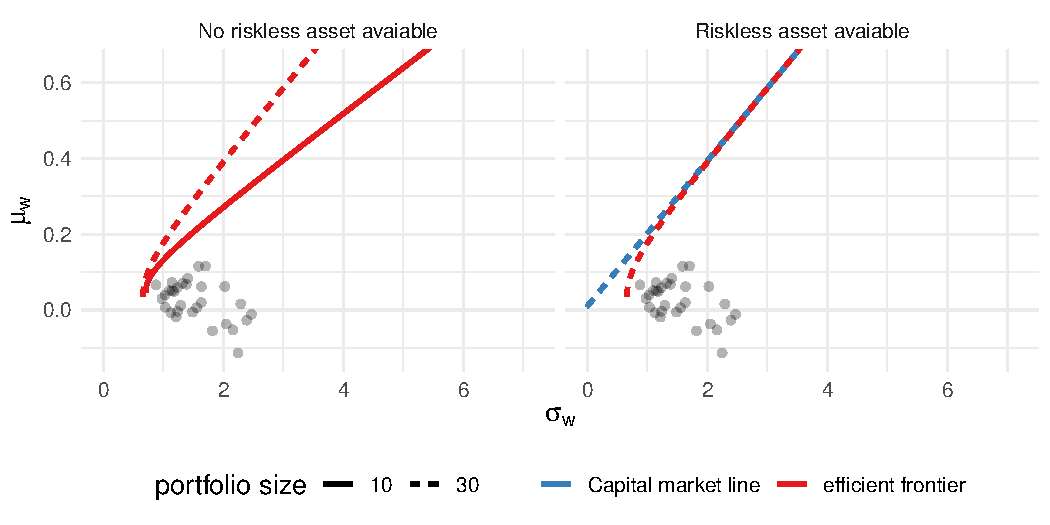
\includegraphics[width=\maxwidth]{figure/mertons_efficient_frontier-1} 

}

\caption[Efficient frontiers without and with a risk-free asset]{Efficient frontiers without and with a risk-free asset. The left plot illustrates two different efficient frontiers for different portfolio sizes. The smaller portfolio is a subset of the larger one. The right plot illustrates the efficient frontier and the capital market line which appears when a risk-free asset is available. The stocks are randomly selected from the S\&P500. The individual means and standard deviations are displayed as points.}\label{fig:mertons_efficient_frontier}
\end{figure}

\end{knitrout}
Figure \ref{fig:mertons_efficient_frontier} displays the efficient frontier and the capital market line, which is yet to be described, for two different portfolio sizes. 
As seen in the left plot, increasing the portfolio size shifts the location of the parabola, e.g., moves it to the left, which serves as an illustration of the diversification effect. 
There is no guarantee that an increase in the portfolio dimension increases the return.
Any point on any of the two lines in the left hand-side plot of Figure \ref{fig:mertons_efficient_frontier} corresponds to a certain efficient and optimal portfolio with a specific value of $\mu_0$. 
The points in the two plots depict the expected returns and the standard deviations of a single-stock portfolio. 
As can be seen through the illustration, diversification will always decrease the risk of the portfolio in the MPT framework. 
No single-stock portfolio can outperform any of the portfolios on the efficient frontier. 

The right hand-side plot of Figure \ref{fig:mertons_efficient_frontier}, displays the efficient frontier and the capital market line.
The capital market line is the solution to an extension to the mean-variance problem.
It displays what happens when a risk-free asset is included in the portfolio allocation problem. 
The risk-free asset is added to the portfolio as any other asset, with the exception that it is deterministic.
With the option to invest in a risk-free asset, the return of the portfolio is $w_0 r_f + \bw^\top \by$. 
The MV problem from \eqref{eqn:mean_variance} is then equal to
\begin{equation}\label{eqn:mean_variance_riskfree}
\begin{aligned}
& \underset{\bw}{\text{minimize}} 
& & \bw^\top \bSigma \bw \\
& \text{subject to}
& & w_0 + \bw^\top \ones = 1 \\
& && w_0 r_f + \bw^\top \bmu = \tilde\mu_0. \\
\end{aligned}
\end{equation}
However, since $w_0 + \bw^\top \ones=1$ the amount invested in the risk-free asset can be substituted by $w_0=1-\bw^\top \ones$.
The problem in \eqref{eqn:mean_variance_riskfree} reduces to an unconstrained optimization problem. 
Its solution is given by 
\begin{equation}\label{eqn:w_mean_variance_riskfree}
  \bw_{TP} = \frac{(\tilde\mu_0-r_f)}{(\bmu-r_f \ones)^\top \bSigma^{-1} (\bmu-r_f \ones)} \bSigma^{-1} (\bmu-r_f \ones).
\end{equation}
The collection of portfolios given by \eqref{eqn:mean_variance_riskfree} defines the whole capital market line which is shown in Figure \ref{fig:mertons_efficient_frontier}. 
The portfolio has many interesting properties. 
If there is a risk-free asset, then there is a possibility to increase the return and decrease the risk of the portfolio. 
This is most easily explained by the efficient frontier, displayed in Figure \ref{fig:mertons_efficient_frontier}. 
For a given level of risk a portfolio can always get the same, and sometimes larger, return! 

The same solution can be obtained from the optimization problem with the quadratic utility, defined as 
$$\min_{\bw} \bw^\top (\bmu- r_f\ones) - \frac{\gamma}{2} \bw^\top \bSigma \bw$$ 
for some $\gamma > 0$.
The solution is given by 
\begin{equation}\label{eqn:TP_def}
  \frac{1}{\gamma}\bSigma^{-1} (\bmu-r_f \ones)
\end{equation}
which coincide with \eqref{eqn:w_mean_variance_riskfree} if 
$$\frac{1}{\gamma} = \frac{(\tilde\mu_0-r_f)}{(\bmu-r_f \ones)^\top \bSigma^{-1} (\bmu-r_f \ones)}.$$ 
The difference is that \eqref{eqn:w_mean_variance_riskfree} depends on a number of parameters while $\gamma$ is a fixed constant.
This is quite common in MPT and there are many portfolio allocation problems which result in the same solution, see, e.g., \citet{bodnar2013equivalence}.

There are many types of risk-free assets.
Ever since the end of 2014, overnight deposit rates (which are risk-free) have been very small in a number of countries \citep[see, e.g., ]{lopez2020have}.
Sweden is among one of these. 
The ''reporänta'' is another type of risk-free asset. 
Although most investors can not invest in an asset connected to the ''reporänta'', it has been less than or equal to zero in Sweden\footnote{See the following visualization from Riksbanken \url{https://www.riksbank.se/sv/statistik/sok-rantor--valutakurser/reporanta-in--och-utlaningsranta/}}.
For the sake of illustration, assume that $r_f=0$ for an investor.
The portfolio \eqref{eqn:w_mean_variance_riskfree} reduces to $\bw_{TP} = \tilde\mu_0 \bSigma^{-1} \bmu / \bmu^\top \bSigma^{-1} \bmu$ or $\bSigma^{-1}\bmu / \gamma$ from \eqref{eqn:TP_def}. 
The term $\bSigma^{-1} \bmu$ is part of the TP portfolio in \eqref{eqn:TP_def}. 
The risk-free asset discounts the returns and the aversion coefficient (or desired return) scales the positions accordingly.
This portfolio is also a part of expression \eqref{eqn:mean_var_solution} and in turn the efficient frontier, although hidden in the matrix $\bQ$. 
With a little work, \eqref{eqn:mean_var_solution} can be rewritten as
$$
\left(1 - \frac{\mu_0-\R}{\V^2} \R \right) \bw_{GMV} + \frac{\mu_0-\R}{\V} \bSigma^{-1} \bmu.
$$
There are two insights to be drawn from this equation.
The first is that the weights on the efficient frontier is a combination of two portfolios, in this case the GMV and the Tangency portfolio. 
This result is usually known as the Mutual fund theorem, see \citet{tobin1958liquidity}.
All portfolios on the efficient frontier can be studied through these two portfolios, which is why this thesis studies these two at great length.
The second is that the tangent portfolio, where the efficient frontier and the capital market line meet, is given by \eqref{eqn:w_mean_variance_riskfree} with 
$$
\tilde\mu_0 = \R + \frac{\mu_0-\R}{\V} \bmu^\top \bQ \bmu.
$$
It is still possible to compare the portfolios, regardless if there is a risk-free rate or not.
The train of thought is the same if $r_f>0$.
The derivations is therefore left to the reader.

Throughout this section the inverse covariance matrix has been used.
As promised, the assumptions that are imposed on it will be discussed in the next section.

\section{Relationship between assets and the (inverse) covariance matrix}\label{sec:cov_prec_matrix}
%%% ----------------------
The covariance matrix $\bSigma$ and the precision matrix $\bSigma^{-1}$ are fundamental to mean-variance portfolio theory. 
This section goes into some depth on the assumptions and restrictions that are placed on the covariance matrix.

For a vector $\by$ with finite second moment, the covariance matrix is defined as $\bSigma=\optn{E}((\by - \bmu)(\by - \bmu)^\top)$. 
It contains the variances of each individual element of $\by$ on the diagonal as well as the covariances between every pair of elements on the off-diagonal. 
That is, each diagonal element corresponds to the univariate case with variance equal to $\optn{E}((y_i - \mu_i)^2)$. 
In the univariate case, a distribution is usually called degenerate or singular if the variance is equal to zero. 
In the multivariate case, the covariance matrix can be singular for a number of reasons. 
It is not limited to the diagonal elements.
This is due to the fact that covariances are involved on the off-diagonal.
There is a need for a broader definition of singularity in multivariate distributions, which can be formulated in terms of positive or positive semidefinite matrices. 

A real symmetric $p\times p$ matrix $\bA$ is called positive definite if $\bz^\top \bA \bz > 0$ or positive semidefinite if $\bz^\top \bA \bz \geq 0$ for all nonzero vectors $\bz \in \mathbbm{R}^p$ (see, e.g., \citet[ch 14.2]{harville1997matrix}).
Let $\bA > 0$ or $\bA \geq 0$ denote a positive or positive semidefinite matrix $\bA$. 
The concept of a singular or degenerate distribution is replaced by a quadratic form.
It involves the covariance matrix of a multi- or matrixvariate distribution.
The definition of positive or positive semidefiniteness can be quite cumbersome to work with. 
The conditions need to hold for all vectors $\bz$. 
A necessary condition for a matrix to be positive definite can be derived using the eigenvalues of a matrix and its eigenvalue decomposition, as described in \citet[ch. 21]{harville1997matrix}.
The eigenvalues, or characteristic roots (with multiplicity), are given by the solutions to
\begin{equation}\label{def:eigenvalue} 
	\left|\bA - \lambda \bI\right| = 0
\end{equation}
where $|\cdot|$ is the determinant of a matrix.
Let $\lambda_i$, $i=1,2,...,p$, denote the \textit{ordered} eigenvalues of the matrix $\bA$ such that $\lambda_1\geq \lambda_2 \geq ... \geq \lambda_p$.
Given an eigenvalue $\lambda_i$, the eigenvectors $\bu_i$ are defined by $\bA \bu_i = \lambda_i \bu_i$, $i=1,2,...,p$. 
Let $\boldsymbol{\Lambda} = \operatorname{diag}(\lambda_1, \lambda_2,...,\lambda_p)$ and $\bU= (\bu_1^\top, \bu_2^\top, ..., \bu_p^\top)^\top$. 
The relation between the matrix $\bA$ and its eigenvalues and eigenvectors can also be written as 
\begin{equation}\label{eqn:eigenvalue_decomp}
	\bA = \bU \boldsymbol{\Lambda} \bU^\top
\end{equation}
which is called the eigen or spectral decomposition.
A necessary condition for a matrix to be positive definite can be directly obtained from the eigenvalue decomposition. 
Let $\bz\in \mathbbm{R}^p$ and $\ba := \bU^{\top} \bz \in \mathbbm{R}^p$, then $\bz^\top \bA \bz = \bz^\top \bU \boldsymbol{\Lambda} \bU ^{\top} \bz = \ba^\top \boldsymbol{\Lambda} \ba = \sum_i^p \lambda_i a_i^2$ which is a second degree polynomial. 
If the eigenvalues are all positive, then necessarily the matrix is positive definite. 
If there are some eigenvalues which are zero, then the matrix is positive semidefinite. 

All papers in this thesis assume that the true covariance matrix is positive definite. 
The assumption has a very important economical interpretation.
If one (or more) eigenvalue(s) are zero, then there is a possibility to construct a portfolio which does not contain any risk.
It is an arbitrage opportunity unless the elements of $\bmu$ are all zero.
Assume $\lambda_p=0$, let $\bu_p$ be its eigenvector and set $\bw = \bu_p / \sum_i^p u_{ip}$. 
The variance of this portfolio is zero since all eigenvectors are orthonormal and its mean is $\bw^\top \bmu$.
If the true covariance matrix is not positive definite there might exist arbitrage opportunities, e.g., the possibility of making profit without taking any risk.

%%%%%% ------------------------------------------------------------------------
\chapter{Statistical models and inference}\label{ch:estim}
%%%%%% ------------------------------------------------------------------------


To \textit{pratically} use the portfolios described by \eqref{eqn:mean_var_solution} the two parameters $\bmu$ and $\bSigma$ have to be specified. 
To specify the parameters manually is not feasible if the portfolio contains many assets.
The mean vector $\bmu$ contains $p$ parameters and the covariance matrix $\bSigma$ contains $p(p+1)/2$ parameters.
If $p=15$ then there is a total of $135$ parameters to specify. 
If there is an informed opinion of the parameters $\bmu$ and $\bSigma$, then using these instead of the true parameters might result in good or bad performance over a given time period, regardless of how performance is defined.
However, they will always be wrong unless they are exactly right from the start.
Therefore, the parameters are usually estimated through data.
If there is enough data and the model is good enough, then the estimates might be very close to true parameters.
They will be more volatile than the manually specified parameters but they at least have the opportunity to converge to the true parameters of interest in the end.
The papers in this thesis combine both but most often relies on data to estimate the parameters of interest.

The data that is used in this thesis are prices for the individual assets.
Let $p_{i,t}$ be the asset price of the $i$th asset at time $t$. 
The methods of this thesis rarely use the asset prices themselves but a transformation of the relative differences, that is, their simple and log-returns. 
The simple return is defined as $r_{i,t} := (p_{i,t}-p_{i,t-1})/p_{i,t-1}$ and the log-return is then defined as $y_{i,t} := \log(r_{i,t} + 1)$ and $\by_t=(y_{1,t},y_{2,t},..., y_{p,t})$.
The return of a portfolio with $p$ assets is modeled as $\bw^\top \by_t$ where $\bw=(w_1, ..., w_p)$ are the portfolio weights.
This is an approximation.
In reality the portfolio return should be $\sum_{i=1}^p w_i r_{i,t}$, which is additive in the number of assets.
However, logarithmic returns are additive in time which can be desirable. 
Compounding returns is simple addition and the approximation can make the statistical analysis more tractable. 
The difference between using $r_{i,t}$ and $y_{i,t}$ is very small if the returns are small since $y_{i,t}=\log(1+r_{i,t}) \approx r_{i,t}$ for small values of $r_{i,t}$.
This is often true for financial assets over short time periods, see \citet[p. 5]{tsay2005analysis}. 

There are many ways to estimate $\bmu$ and $\bSigma$.
The most simple and versatile method is the Method of Moments (MM) (see e.g., \citet[ch. 9]{wasserman2004all}). 
Let $\bY = (\by_1, \by_2, ..., \by_n)$ be a sample of log-returns.
Using the sample, $\bmu$ and $\bSigma$ are replaced with the sample mean and the sample covariance matrix, i.e.,
$$
\byb = \frac{1}{n} \sum_i^n \by_i, \; \bS = \frac{1}{n}\bY \left(\bI_n - \frac{1}{n} \ones_n \ones_n^\top \right) \bY^\top.
$$
This is always a feasible approach assuming that the first two moments actually exist. 
However, it introduces some issues.
If the sample size $n$ is small, then the estimates are naturally imprecise.
Furthermore, MPT relies on $\bSigma^{-1}$ and not $\bSigma$.
For the sample covariance matrix to be positive definite, it demands that $n>p$, which introduces more constraints on the estimates.
It is natural to ask: does an imprecise estimate of the covariance matrix $\bSigma$ provide an equally imprecise estimate of the inverse $\bSigma^{-1}$?
In some simple cases the answer is no, sometimes it is worse. 
It is therefore very important to understand the implications of not using the true parameters but their sample counterparts.
In other words, it is important to understand the effect of estimation uncertainty.
There are many approaches to this but the most natural is the bottom-up approach. 
If the asset returns $\bY$ follows some distribution, then there is potentially some statistical properties for $\byb$ and $\bS$.
The aim is then to understand the implications of using $\bS^{-1}$ instead of $\bSigma^{-1}$ and $\byb$ instead of $\bmu$ in \eqref{eqn:mean_var_solution} and all the corresponding moments.
To investigate how estimation uncertainty affects the methods from MPT the next section introduces the models that are used in this thesis.
Their properties that are used in this thesis, are stated in the coming sections.
Thereafter the implications of using estimates for MPT are discussed in brief.

\section{Matrixvariate distributions}
One of the most fundamental models for asset returns is the multivariate normal distribution. 
Since most of the distributions in this thesis are matrixvariate, the matrixvariate normal distribution is presented. 
It is slightly more general than the multivariate normal distribution. 
The matrixvariate distribution can capture more structure in the data than its multivariate counterpart.
Let $\otimes$ denote the Kronocker product, the matrixvariate normal distribution is defined as
% Multivariate normal distribution
\begin{definition}[Definition 2.2.1 in \citet{GuptaNagar2000}]\label{def:matrixnormal}
	The random matrix $\bY$ $(p \times n)$ is said to have a matrixvariate normal distribution with mean matrix $\bM$ and covariance matrix $\bSigma \otimes \bGamma$ where $\bSigma > 0$ is of dimension $(p \times p)$ and $\bGamma >0$ is of dimension $(n \times n)$, if $\optn{vec}(\bY^\top) \sim N_{n,p}(\optn{vec}(\bM^\top), \bSigma \otimes \bGamma)$.
\end{definition}
The multivariate normal distribution is a simple special case of it with $n=1$ and $\bGamma = \bI$.
Since each element in $\bY$ has support on the real line the most natural thing is to use this type of model for the log-returns of the assets.
A property of the matrixvariate normal distribution is that it is closed under linear transformations.
That plays an important role for determining the distribution of the estimator $\byb$ but also to determine the portfolio return distribution.
Both are linear transformations.
%The matrixvariate normal distribution is very often used and the applications are many.
However, \citet{cont2001empirical} described a number of stylized facts of log-returns. 
These stylized facts describe the characteristics of asset returns on different frequencies.  
It is argued that the multivariate normal distribution has too thin tails in comparison to what is usually observed in asset returns on higher frequencies.
Cont argued that daily returns are usually not symmetric and often show volatility clustering.
However, Cont also argued that returns on a lower frequency such as monthly or quarterly can be close to normal.
The shape of the return distribution is not the same over different frequencies. 
A motivation for the matrixvariate normal distribution can be thought of as an investor which invests in the portfolio infrequently.
That does not mean that he/she cannot observe the results of the market on a higher frequency!

In the univariate case the properly normalized sample variance follows a chi-square distribution assuming that the returns follow a normal distribution. 
If the returns follow a multivariate normal distribution and are assumed to be independent, then $\bS$ follows what is known as a Wishart distribution. 
It is essentially a generalization of the chi-square distribution. 
The probability density function (p.d.f.) of a Wishart distribution is given below.
% Wishart
\begin{definition}[Definition 3.2.1 in \citet{GuptaNagar2000}]\label{def:wishart}
	A $p\times p$ random symmetric positive definite matrix $\bS$ is said to have a Wishart distribution with parameter $n$ ($n\geq p$) and $\bSigma > 0$, $(p \times p)$ written as $\bS \sim W_p(n, \bSigma)$ if its p.d.f. is given by
	\begin{equation}\label{eqn:wishart_density}
  	\frac{|\bS|^{(n-p-1)/2} |\bSigma|^{- n/2} }{2^{pn/2} \Gamma_p (n/2) } \exp\left\{-\frac{1}{2} \operatorname{tr}(\bSigma^{-1}\bS)  \right\}
	\end{equation}
	where $ \Gamma_p (\cdot) $ is the multivariate gamma function.
\end{definition}
In comparison to the normal distribution the Wishart distribution is used very frequently as a model for covariance matrices, although in a slightly different context.
The model is very often used for realized covariance matrices, see \citet{barndorff2004econometric}, \citet{golosnoy2019exponential} or \citet{alfelt2021modeling}.
A realized covariance matrix is an estimate of the volatility process from returns on a much higher frequency than what is used in this thesis.

If $\bY \sim N_{p,n}(\bmu \ones_n^\top, \bSigma \otimes \bI_n)$, then $n\bS \sim W_p(n-1, \bSigma)$ by \citet[Theorem 3.3.6 in]{GuptaNagar2000}.
Working from the bottom-up there is now a model for the estimated parameters of the original model.
As previously stated, MPT works with inverse covariance matrices and not with the covariance matrix itself. 
Thankfully, the Wishart distribution has an inverse counterpart.
% Inverse Wishart
\begin{definition}[Definition 3.4.1 in \citet{GuptaNagar2000}]\label{def:inverse_wishart}
	A random matrix $\bV$ is said to be distributed as an inverted Wishart distribution with $m$ degrees of freedom and parameter matrix $\bGamma$ $(p \times p)$, denoted by $\bV \sim IW_p(m, \bGamma)$, if its density is given by
	\begin{equation}\label{eqn:inverse_wishart}
	\frac{2^{-(m-p-1)p/2} |\bGamma|^{(m-p-1)/2} }{\Gamma_p ((m-p-1)/2) |\bV|^{m/2}} \exp\left\{ -\frac{1}{2} \bV^{-1} \bGamma \right\}, \; m > 2p, \bV, \bGamma > 0.
	\end{equation}
\end{definition}
To once more connect to the univariate setting, the inverted sample variance follows an inverted chi-square distribution which is a special case of the inverted gamma distribution.
It is only natural that the inverted Wishart matrix is a matrix variate generalization of the inverted gamma distribution (\citet[page 111]{GuptaNagar2000}). 
It demands quite specific constraints on the parameters of the model, namely $m > 2p$.
This is a hint to an answer that was posed in the beginning of this section, does the inverse change estimation uncertainty? 
The constraint $m>2p$ provides a partial answer that \textit{something} changes with the properties of $\bS$ when taking inverses.
The constraints of the model are more strict.
From Theorems 3.3.7 and 3.4.1, and Theorem 3.4.3 of \citet{GuptaNagar2000} the first moments of the two are
$$
\optn{E}\left[\bS\right] = \frac{n-1}{n} \bSigma, \; 
\optn{E}\left[\bS^{-1}\right] = \frac{n}{n-p-2}\bSigma^{-1}.
$$
If $n$ is sufficiently large, then the sample covariance matrix is (close to) unbiased.
That is not necessarily the case for its inverse.
If an investor believes in diversification, then he/she should own many assets, e.g., $p$ should be large.
That in turn could make the estimator very biased!
Inverses can potentially make matters worse.

%Furthermore, the noise in the sample mean can be extremely large in comparison to the noise in the sample covariance matrix.
%The weights from \eqref{eqn:mean_var_solution} will be much more noisy whenever $\mu_0 \neq \R$ since these will depend on the sample mean vector (see e.g., \citet{merton1980estimating}, \citet{chopra1993effect}).
%It is perhaps one of the most common motivations for using the GMV portfolio.
It has been well established that returns on a high frequency does not follow a normal distribution. 
The next feature, and perhaps most natural, to include is skewness of the asset returns and to assess its effect on portfolios. 
A $p$ dimensional Closed Skew Normal (CSN) random vector $\bz$ has density
\begin{equation}
  f_\bz(\ba; \bmu, \bSigma, \bD, \bv, \Delta) = C \phi_p(\ba; \bmu, \bSigma) \Phi_q(\bD(\ba-\bmu); \bv, \Delta)
\end{equation}
where $C$ is a normalization constant, $\phi_k$ and $\Phi_k$ are the probability density and cumulative distribution function for a $k$-dimensional standard normal distribution and $\bmu, \bSigma, \bD, \bv$ and $\Delta$ are parameters of appropriate dimensions. 
Its matrixvariate counterpart is simply defined through the vec operator. 
% Closed skew normal distribution
\begin{definition}[Definition 3.1 in \citet{dominguez2007matrix}]
  A random matrix $\bY$ $(p \times n)$ is said to have a matrix variate closed skew-normal distribution with parameters $\bM$ $(p \times n)$, $\bA$ $(np \times np)$, $\bB$ $(nq \times mp)$, $\bL$ $(q \times m)$ and $\bQ$ $(mq \times mq)$, with $\bA > 0$ and $\bQ>0$ if
  \begin{equation}
    \optn{vec}(\bY^\top) \sim CSN_{pm, qn}\left(\optn{vec}(\bM^\top), \bA, \bB, \optn{vec}(\bL^\top), \bQ\right).
  \end{equation}
\end{definition} 
The closed skew-normal distribution is heavily parametrized. 
For each column in the matrix $\bY$ there is a mean vector $\bm$ and an additional four vectors $\ba$, $\bb$, $\bl$ and $\bq$ describing skewness and volatility of the asset returns.
The matrixvariate distribution can capture a lot of structure.
However, it also puts a heavy restriction on some of the parameters, as they need to be positive definite.
The parameter $\bA$ might be interpreted as a covariance matrix although this is a simplification.
It is something more and can capture variance along \textit{both} axes of the matrix $\bY$, such as volatility for a specific asset but also unconditional volatility over time.
There is also some type of dependence between $\bA$ and how skewness is observed, by the fact that moments include \textit{almost all of the parameters} (see, e.g., the steps that begins at the end of page 1606 in \citet{dominguez2007matrix}).
Due to the stochastic representation in Proposition 2.1 \citet{dominguez2007matrix}, the introduction of skewness can be thought of as random shocks to the mean.
The overzealous parametrisation makes estimating the parameters rather difficult and that is why paper \hyperref[sec:paper2]{2} uses the assumption that $q=m=1$.

The last model in this thesis is the most general.
It is also the model that has the least amount of interesting properties in itself.
It is the following location and scale model
\begin{equation}\label{eqn:location_scale_model}
\bY \eqdist \bmu \ones^\top_n + \bSigma^{1/2} \bZ
\end{equation}
where $\eqdist$ stands for equality in distribution  and $\bZ = \{z_{ij}\}$, $i=1,2,...,p$, $j=1,2,...,n$.
Equality in distribution is a synonym for a stochastic representation.
A stochastic representation has the possibility to break down a distribution in terms of smaller and simpler random variables. 
The most simple case is the t distribution, which can be described by the ratio of a chi-square distribution and a random normal variable.
The stochastic representation would be written as $t \eqdist z \sqrt{(f-1)/\chi}$ where $z$ is a standard normal random variable, $\chi$ a chi-squared random variable with $f$ degrees of freedom independent of $z$.
It is very common to assume moment conditions on $z_{ij}$, such as finite fourth moment or potentially $4+\epsilon$ finite moment, for some $\epsilon>0$.
Although the model can capture many types of return distributions, such as skew, heavy tailed and sometimes even heteroscedasticity, there is very little to say about it.

Estimates of model parameters are interesting in themselves. 
However, this thesis is about portfolios.
In the next section, the implications of estimation uncertainty on optimal portfolios are displayed.

\section{Inference and sampling distributions of optimal portfolios and their characteristics}
The empirical counterpart of \eqref{eqn:mean_var_solution} is obtained by replacing $\bmu$ and $\bSigma$ with $\byb$ and $\bS$. It is equal to
\begin{equation}\label{eqn:meanvar_solution_sample}
	\hbw_{MV} = \frac{\bS^{-1}\ones}{\ones^\top \bS^{-1}\ones} + \frac{\mu_0 - \hR}{\hV} \hat{\bQ} \byb,\; \hat{\bQ} = \bS^{-1} - \frac{\bS^{-1} \ones \ones^\top \bS^{-1}}{\ones^\top \bS^{-1} \ones}
\end{equation}
where 
\begin{equation}\label{eqn:meanvar_characteristics_sample}
  \hV = \frac{1}{\ones^\top \bS^{-1}\ones},\; \hR = \frac{\ones^\top \bS^{-1} \byb}{\ones^\top \bS^{-1}\ones}
\end{equation}
and the shape parameter of the efficient frontier $\hat{s} = \byb^\top \bQ \byb$.
This is a portfolio that can actually be invested in. 

From the previous section, the distributions of $\byb$ and $\bS$ are known if $\bY$ follows the matrixvariate normal distribution stated in Definition \ref{def:matrixnormal}. 
In this scenario, the two estimators are even independent (see Theorem 3.3.6 in \citet{GuptaNagar2000}) which makes the analysis simpler.
However, in MPT there are many complicated transformations containing both $\byb$ and $\bS^{-1}$.
One example is the return for the GMV portfolio
\begin{equation}\label{eqn:return_gmv_sample}
\hR=\frac{\byb^\top\bS^{-1}\ones}{\ones^\top\bS^{-1}\ones}.
\end{equation}
Since $\byb$ and $\bS$ are independent, the conditional distribution of \eqref{eqn:return_gmv_sample} given $\byb=\tilde\by$ is the same as the unconditional distribution of $\tilde{R}_{GMV} = \tilde\by^\top \bS^{-1} \ones / \ones^\top \bS^{-1} \ones$.
However, \eqref{eqn:return_gmv_sample} still contains the sample covariance matrix in the nominator as well as the denominator.
The two quantities $\byb^\top\bS^{-1}\ones$ and $\ones^\top\bS^{-1}\ones$ are obviously not independent.
To solve the problem at hand consider two $p\times p$ matrices with the following block structure 
\begin{equation}\label{eqn:blockmat}
\bA = \begin{pmatrix}
       \bA_{11} & \bA_{12} \\
       \bA_{21} & \bA_{22}
      \end{pmatrix},\;
\bV = \begin{pmatrix}
           \bV_{11} & \bV_{12} \\
           \bV_{21} & \bV_{22}
          \end{pmatrix}
\end{equation}
where $\text{dim}(\bA_{11}) = \text{dim}(\bV_{11})= m \times m$, $m<p$. 
Let $\bA_{11\cdot 2} := \bA_{11} - \bA_{12} \bA_{22}^{-1} \bA_{21}$ denote the Schur complement of the matrix $\bA$ and define $\bV_{11\cdot 2}$ in the same manner. 
The following theorem is used a lot in papers \hyperref[sec:paper2]{1} and \hyperref[sec:paper2]{2}.
\begin{theorem}[Theorem~3 in \citet{BodnarOkhrin2008}]\label{thrm:invWis}
 Suppose $\bA \sim W^{-1}_k(n, \bV)$, where $\bA$ and $\bV$ are partitioned as in \eqref{eqn:blockmat}. Then
 \begin{enumerate}[(a)]
	\item $\bA_{11\cdot 2} \sim W^{-1}_m(n-k+m, \bV_{11\cdot 2})$ and is independent of $\bA_{22}$;
 	\item $\bA_{12} | \bA_{22}, \bA_{11\cdot 2} \sim \mathcal{N}(\bV_{12}\bV^{-1}_{22} \bA_{22}, \bA_{11\cdot 2} \otimes \bA_{22} \bV^{-1}_{22} \bA_{22})$;
	\item $\bA_{22} \sim W^{-1}_{p-m} (n-2m, \bV_{22})$;
	\item $\bA_{12}\bA^{-1}_{22}$ is independent of $\bA_{22}$, with density given by 
	\begin{flalign}
            f_{\bA_{12}\bA^{-1}_{22}}(\bX) = & \frac{  |\bV_{11\cdot 2}|^{-\frac{1}{2} (p-m)} |\bV_{22}|^{\frac{1}{2}m}  }{ \pi^{\frac{(p-m)m}{2}} } \frac{\Gamma_{m} \left(\frac{n-m-1}{2} \right)}{\Gamma_{m} \left(\frac{n-p-1}{2} \right)} \nonumber \\
            & \times \left|\bI + \bV^{-1}_{11\cdot 2} \left(\bX - \bV_{12}\bV_{22}^{-1} \right)\bV_{22} \left(\bX - \bV_{12}\bV_{22}^{-1} \right)^\top  \right|^{-\frac{1}{2}(n-m-1)} \label{eqn:almostT}
	\end{flalign}
	where $\Gamma_{m}(\cdot)$ is the multivariate Gamma function;
	\item $\bA_{22}$ is independent of $\bA_{12}\bA^{-1}_{22}$ and $\bA_{11\cdot 2}$;
	\item $\bA_{11\cdot 2}| \bA_{12}\bA^{-1}_{22}=\bX \sim W_m^{-1}(n,  \bV_{11\cdot 2} + \left(\bX - \bV_{12}\bV_{22}^{-1} \right)\bV_{22} \left(\bX - \bV_{12}\bV_{22}^{-1} \right)^\top )$.
 \end{enumerate}
\end{theorem}
Given an inverse Wishart distribution the distribution of many, quite difficult, transformations of its sub-matrices can be derived. 
Let $\bH^\top = (\bL^\top, \tilde\by, \ones)^\top$ and note that $(\bH \bS^{-1} \bH^\top)^{-1}$ follows a Wishart distribution by Theorem 3.3.13 in \citet{GuptaNagar2000}. 
The inverse of $(\bH \bS^{-1} \bH^\top)^{-1}$ follows an inverse Wishart distribution.
Observe that
$$
\bH \bS^{-1} \bH^\top = 
\begin{pmatrix}
  \bL \bS^{-1} \bL^\top & \bL \bS^{-1}\tilde\by& \bL \bS^{-1} \ones \\
  \tilde\by^\top \bS^{-1} \bL^\top & \tilde\by^\top \bS^{-1}\tilde\by & \tilde\by^\top \bS^{-1} \ones \\
   \ones^\top \bS^{-1} \bL^\top& \ones^\top \bS^{-1}\tilde\by & \ones^\top \bS^{-1} \ones  \\
\end{pmatrix}.
$$
If $\bA_{12}=(\bL \bS^{-1} \ones \; \tilde\by^\top \bS^{-1} \ones)^\top$ and $\bA_{22}^{-1}=1/\ones^\top \bS^{-1} \ones$, then, together with Theorem \ref{thrm:invWis} results in
$$
\bA_{12}\bA^{-1}_{22}= 
\begin{pmatrix}
  \frac{\bL^\top \bS^{-1} \tilde \by}{\ones^\top \bS^{-1} \ones} &
  \frac{\tilde\by^\top \bS^{-1} \ones}{\ones^\top \bS^{-1} \ones}
\end{pmatrix}^\top
$$
which is the joint distribution of the return of the GMV portfolio, $\hR$, and some scaled version of linear combinations of the TP with $\gamma = \hV^{-1}$ and $r_f=0$.
By \eqref{eqn:almostT} the joint distribution of these follows a matrixvariate t-distribution (see \citet[Definition 4.2.1 in]{GuptaNagar2000}) and the return of the GMV portfolio is independent to its variance. 
Similar to the matrixvariate normal distribution, the matrixvariate t-distribution is also closed under linear transformations (see \citet[Theorem 4.3.5 in]{GuptaNagar2000}).
This implies that $\hR$ follows a t-distribution, conditionally on the mean.
The parameters of the distribution are presented in Lemma 7.1 in paper \hyperref[sec:paper1]{1}. 
Paper \hyperref[sec:paper1]{1} uses these properties to derive the full joint distribution for all the quantities used in \eqref{eqn:meanvar_solution_sample}.
It even provides the joint distribution of all optimal portfolios. 
The joint distribution is characterized through its stochastic representation.
The stochastic representation is a very verbose way of characterizing the distribution in terms of simple random variables.
These random variables are simple to simulate.
Any quantity of interest from the joint distribution can simply be computed through Monte Carlo approximation. 
For some methods, simulations are the only way to compute the quantities of interest.
It can therefore be very important that simulations are fast.
This is extremely simple to do with the stochastic representation.

\section{Simulations, inverses and why stochastic representations are valuable}
Assume that an investor is interested in the GMV portfolio and to have some disposition of what some possible values of the true covariance matrix may be.
In this scenario it is also assumed that the returns follow a matrixvariate normal distribution, i.e. $\bY \sim N_{p,n}(\bmu \ones_n^\top, \bSigma \otimes \bI_n)$. 
To simulate from the sampling distribution of the variance of the GMV portfolio, there are a number of steps that needs to be performed
\begin{enumerate}
  \item Simulate $\bY$ and construct $\bS$
  \item Invert $\bS$
  \item Compute $\hV$
\end{enumerate}
The second step is notoriously demanding.
The default method to use in R is 'solve' which is a wrapper for certain LAPACK\footnote{For the interested reader \url{https://www.netlib.org/lapack/}} functions.
The inverse itself takes $2p^3$ flops (cpu cycles), which is not cheap (see, e.g., \citet[ch. 14]{higham2002accuracy}).
If $p$ is large, then simulation of the quantity $\hV$ will be extremely cumbersome.
Another method is R's \hlstd{chol2inv} which relies on the Cholesky decomposition. 
In theory, it should be faster but demands that the Cholesky decomposition is computed.
The last two options that are available is to simulate $\bS$ directly or to derive the stochastic representation of $\hV$.
Papers \hyperref[sec:paper1]{1} and \hyperref[sec:paper2]{2} go into great detail to derive the stochastic representation of different quantities of optimal portfolios. 
One of them is the sample variance of the GMV portfolio.
If $\bY \sim N_{p,n}(\bmu \ones_n^\top, \bSigma \otimes \bI_n)$, then by Theorem 1 in \citet{bodnar2020sampling} $\hV \sim \V\xi /(n-1)$ where $\xi \sim \chi^2_{n-p}$.
The inversion can be omitted all together.
In \ref{benchmark} there is some R-code which implements a small benchmark to highlight why these types of representations can be really valuable.
\begin{knitrout}\small
\definecolor{shadecolor}{rgb}{1, 1, 1}\color{fgcolor}\begin{kframe}
\captionof{chunk}{R-code for benchmarking different simulation approaches of the variance of the GMV portfolio.}\label{benchmark}\begin{alltt}
\hlcom{# setup}
\hlstd{p} \hlkwb{<-} \hlnum{150}
\hlstd{n} \hlkwb{<-} \hlnum{250}
\hlstd{Sigma} \hlkwb{<-} \hlstd{HDShOP}\hlopt{::}\hlkwd{RandCovMtrx}\hlstd{(p)}
\hlstd{Sigma_chol} \hlkwb{<-} \hlkwd{chol}\hlstd{(Sigma)}
\hlstd{mu} \hlkwb{<-} \hlkwd{runif}\hlstd{(p,} \hlopt{-}\hlnum{0.1}\hlstd{,} \hlnum{0.1}\hlstd{)}
\hlstd{Sigma_inv} \hlkwb{<-} \hlkwd{solve}\hlstd{(Sigma)}
\hlstd{V_GMV} \hlkwb{<-} \hlnum{1}\hlopt{/}\hlkwd{sum}\hlstd{(Sigma_inv)}
\hlcom{# microbechmark}
\hlstd{result} \hlkwb{<-} \hlkwd{microbenchmark}\hlstd{(}
  \hlcom{# Simulate Y directly, construct S, invert and compute GMV variance}
  \hlkwc{`Scenario 1`} \hlstd{= \{}
    \hlstd{Y} \hlkwb{<-} \hlstd{mu} \hlopt \hlkwd{t}\hlstd{(}\hlkwd{rep}\hlstd{(}\hlnum{1}\hlstd{,n))} \hlopt{+} \hlkwd{t}\hlstd{(Sigma_chol)}\hlopt\hlkwd{matrix}\hlstd{(}\hlkwd{rnorm}\hlstd{(n}\hlopt{*}\hlstd{p),} \hlkwc{ncol} \hlstd{= n)}
    \hlstd{S} \hlkwb{<-} \hlkwd{var}\hlstd{(}\hlkwd{t}\hlstd{(Y))}
    \hlnum{1}\hlopt{/}\hlkwd{sum}\hlstd{(}\hlkwd{solve}\hlstd{(S))}
  \hlstd{\},}
  \hlcom{# Simulate Y directly, construct S and its chol. decomp., use chol2inv and}
  \hlcom{# compute GMV variance}
  \hlkwc{`Scenario 2`} \hlstd{= \{}
    \hlstd{Y} \hlkwb{<-} \hlstd{mu} \hlopt \hlkwd{t}\hlstd{(}\hlkwd{rep}\hlstd{(}\hlnum{1}\hlstd{,n))} \hlopt{+} \hlkwd{t}\hlstd{(Sigma_chol)}\hlopt\hlkwd{matrix}\hlstd{(}\hlkwd{rnorm}\hlstd{(n}\hlopt{*}\hlstd{p),} \hlkwc{ncol} \hlstd{= n)}
    \hlstd{S} \hlkwb{<-} \hlkwd{var}\hlstd{(}\hlkwd{t}\hlstd{(Y))}
    \hlstd{S_chol} \hlkwb{<-} \hlkwd{chol}\hlstd{(S)}
    \hlnum{1}\hlopt{/}\hlkwd{sum}\hlstd{(}\hlkwd{chol2inv}\hlstd{(S_chol))}
  \hlstd{\},}
  \hlcom{# Simulate S directly, invert and compute GMV variance}
  \hlkwc{`Scenario 3`} \hlstd{= \{}
    \hlstd{S} \hlkwb{<-} \hlkwd{rWishart}\hlstd{(}\hlnum{1}\hlstd{,} \hlkwc{df}\hlstd{=n}\hlopt{-}\hlnum{1}\hlstd{,} \hlkwc{Sigma}\hlstd{=Sigma)[,,}\hlnum{1}\hlstd{]}
    \hlnum{1}\hlopt{/}\hlkwd{sum}\hlstd{(}\hlkwd{solve}\hlstd{(S))}
  \hlstd{\},}
  \hlcom{# Simulate directly from the GMV sample variance distribution.}
  \hlkwc{`Scenario 4`} \hlstd{= V_GMV}\hlopt{/}\hlstd{(n}\hlopt{-}\hlnum{1}\hlstd{)} \hlopt{*} \hlkwd{rchisq}\hlstd{(}\hlnum{1}\hlstd{,} \hlkwc{df}\hlstd{=n}\hlopt{-}\hlstd{p),}
  \hlkwc{times}\hlstd{=}\hlnum{1000}
\hlstd{)}
\end{alltt}
\end{kframe}
\end{knitrout}

\begin{knitrout}\small
\definecolor{shadecolor}{rgb}{1, 1, 1}\color{fgcolor}\begin{figure}

{\centering 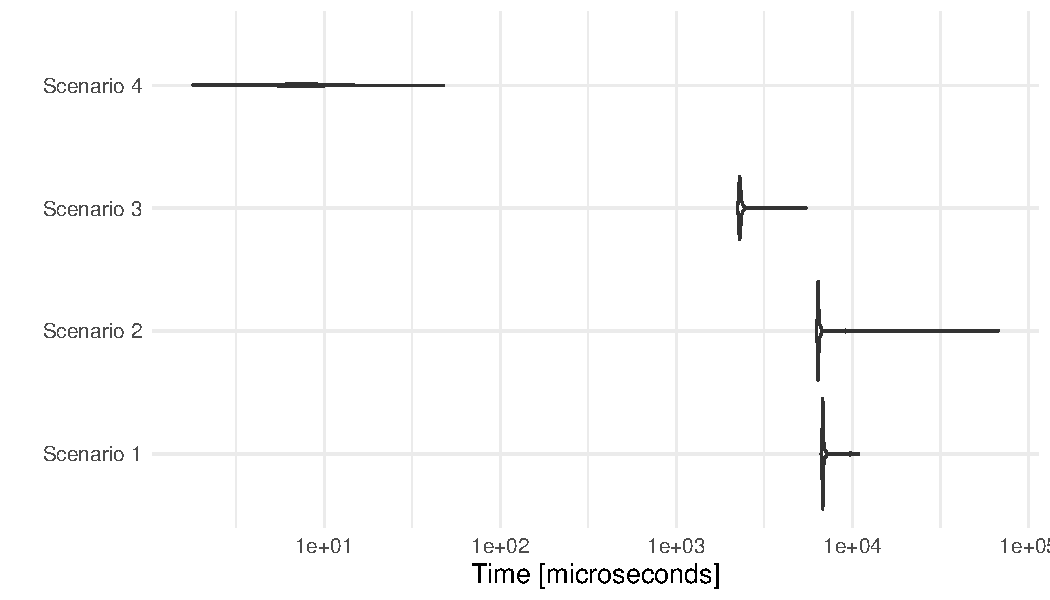
\includegraphics[width=\maxwidth]{figure/microbenchmark_output-1} 

}

\caption[Difference in performance between the simulation methods for the estimated variance of the GMV portfolio based on 1000 simulations]{Difference in performance between the simulation methods for the estimated variance of the GMV portfolio based on 1000 simulations.}\label{fig:microbenchmark_output}
\end{figure}

\end{knitrout}

In Figure \ref{fig:microbenchmark_output} a violinplot of the benchmark is displayed.
Scenario 4 uses the stochastic representation and the time it takes to simulate 1000 observations from the sampling distribution is much smaller any of the former strategies.
It is quite clear that it is the fastest.
Scenario 3 comes in second place in terms of speed.
Simulating directly from the Wishart distribution is quick.
This can partly be explained by the fact that the function `rWishart` calls on another function which is implemented in C, which is very fast.
Scenario 1 and 2 does not make use of C or stochastic representations which make them the slowest.
The conclusion is that inversions are very cumbersome to deal with and take a lot of time regardless if the Cholesky decomposition is used or not.
It can also be a very unstable operation, especially if the matrix is close to singular.
Simulating the variance of the GMV portfolio is one simple example of the application of the stochastic representation.
Using the results from Papers \hyperref[sec:paper1]{1} and \hyperref[sec:paper2]{2} one can perform large scale simulations efficiently to compute moments from the sampling distributions for the portfolio characteristics and the portfolio weights themselves.

A large portion of this thesis works with $\bS$, $\byb$.
This is of course two options out of many.
The estimators $\bS$ and $\byb$ contain a lot of uncertainty where the former contains less than the latter (see, e.g., \citet{frankfurter1971portfolio}, \citet{merton1980estimating}, \citet{best1991sensitivity}). 
Furthermore, there are a number of other issues at hand.
If $p$ is comparable to $n$ but $n>p$, then the expectation of the inverse Wishart distribution is very biased.
It is also very hard to compute $\bS^{-1}$ from $\bS$ numerically if the matrix is close to singular.
There are two strategies to solve the problem.
The first is to understand what implications estimation uncertainty has on the quantities of interest directly.
Papers \hyperref[sec:paper1]{1} and \hyperref[sec:paper2]{2} do so by deriving the sampling distribution of the portfolios.
The second approach is to use another estimator which can limit or decrease the estimation uncertainty.
That will come at a cost.
It may, or will, introduce some bias to the portfolios.
It is something of utmost importance if an investor believes in diversification.

%%%%%% ------------------------------------------------------------------------
\chapter{Diversification, infinitely many assets and shrinkage estimators}\label{ch:highdim}
%%%%%% ------------------------------------------------------------------------


In the previous chapter one specific way of estimating the sample covariance matrix was presented.
If there is a lot of data on the assets that is in the portfolio, then the estimated weights will most likely be close to the correct portfolio.
The estimated portfolio will be consistent, e.g., it estimates the correct object of interest. 
As previously mentioned, diversification is one of the best risk management tool there is and therefore, the asset universe is supposed to be big.
However, \citet{bodnar2016optimal} showed that the out-of-sample variance of the GMV portfolio can behave remarkably bad if $p$ is close to $n$.
The out-of-sample variance for the GMV portfolio is defined as 
\begin{equation}\label{eqn:oot_var}
  \hbw_{GMV}^\top \bSigma \hbw_{GMV} = \frac{\ones^\top \bS^{-1} \bSigma \bS^{-1} \ones }{(\ones^\top \bS^{-1} \ones)^2},
\end{equation}
which tends to $\V/(1-c)$ whenever $p,n \rightarrow \infty$ s.t. $p/n \rightarrow c \in [0,1)$. 
If $c$ is close to one, then the out-of-sample GMV portfolio variance will explode. 
\textit{Estimation uncertainty dominates the diversification effect}.
There are many solutions to the problem at hand (see, e.g., \citet{lw17} and the references therein). 
The solution used in this thesis is Random Matrix Theory (RMT) and the use of some types of shrinkage estimators. 
Both subjects are grand.
A small introduction to them is presented in the following sections.

\section{A short introduction to random matrix theory and the Stieltjes transform}
The subject of RMT has many applications.
It was originally developed in the context of quantum physics (see \citet[Chapter 1 of]{mehta2004random}).
The theory and its applications have since then developed quite a lot.
Many fields, such as combinatorics, computational biology, wireless communication and finance (see, e.g., \citet{livan2018introduction}) use these results.
One of the seminal works in RMT was made by \citet{wigner1967random}. 
Wigner originally modeled the limiting spectral distribution of a $p \times p$ dimensional random matrices $\bX$ with standard normal entries.
The term "standard" might be a little misleading for statisticians as the matrix $\bX$ contains independent random variables although not identically distributed.
The entries on the diagonal are $N(0,2)$ and the entries on the off-diagonal are $N(0,1)$.

This thesis mainly works with symmetric matrices with real entries, e.g. the sample covariance matrix, though it can generalize to any matrix with real eigenvalues, also known as Hermitian matrices.
Since $\bX$ or any other matrix in RMT, e.g. the sample covariance matrix $\bS$, is a sample from a model, it is most natural to define a Empirical Spectral Distribution (ESD) function rather than the classical Cumulative Distribution Function (CDF).
The ESD of a matrix $\bX$ is defined as
$$
F^{\bX}(x)= \frac{1}{p} \sum_{i=1}^p \mathbbm{1}(\lambda_i \leq x)
$$ 
where $\lambda_i$ are the eigenvalues from the eigenvalue decomposition, see section \ref{sec:cov_prec_matrix}.
A central assumption is that if $p \rightarrow \infty$ then the ESD converges to the limiting cumulative distribution function of the spectral distribution of $\bX$, which is simply referred to as the Limiting Spectral Distribution (LSD).
The asymptotics in RMT is slightly different to most common settings.
As $p \rightarrow \infty$, $\bX$ will have infinitely many columns as well as rows.
\citet{wigner1967random} showed that if $\bX$ is a random matrix with standard normal entries then it ESD converges to the following LSD 
$$
F(x) = \begin{cases}
\frac{1}{2\pi} \sqrt{4-x^2} & \text{ if } |x|\leq 2 \\
0 & \text{ otherwise.}
\end{cases}
$$
If the reader is interested in how it is derived, have a look in Chapter 2 of \citet{bai2010spectral}.
There are many interesting facts about the ESD and its LSD. 
One of the most interesting is the support of the LSD.
The normal distribution has unbounded support but the eigenvalues of $\bX$ converges to a distribution with bounded support (see, \citet{livan2018introduction} for a good explanation to the reason why).
This is of course not always the case.
The normal distribution is one of few distributions that has support on the whole real line and all moments.
\citet{burda2002free} show that there can still exist a LSD when the elements of $\bX$ do not have finite second moment.
The LSD can even have closed form solutions.

Although the model Wigner considered is interesting, this thesis exclusively deals with sample covariance matrices which are symmetric.
\citet{marchenko1967distribution} extended the result of \citet{wigner1967random} to the sample covariance matrix.
Assume that $\bX$ is a $p \times n$ matrix that contains i.i.d random variables with zero mean and variance equal to $1$.
The limit is now taken over the two quantities $p$ and $n$ at the same time, such that $p/n$ tends to a constant.
The ratio is usually called the concentration ratio $c$.
In this introduction it is assumed that $c<1$.
The density of the limiting spectral distribution of $\bS=\frac{1}{n} \bX \bX^\top$ was then shown to be
$$
F(x) = \begin{cases}
\frac{1}{2\pi x c} \sqrt{(b-x)(x-a)} & \text{ if } a \leq x \leq b\\
0 & \text{ otherwise}
\end{cases}
$$
where $a=(1-\sqrt{c})^2$ and $b=(1+\sqrt{c})^2$. 
The distribution has, once again, bounded support! 
The eigenvalues seem to attract each other. 
Although the sample covariance matrix appears very often in the context of MPT, it is not the object of interest. 
MPT cares about its inverse, as discussed in Chapter \ref{ch:MPT}, which the Stieltjes transform can help with. 
The Stieltjes transform of a function $F: \mathbbm{R} \rightarrow \mathbbm{R}$ is defined as 
\begin{equation}\label{eqn:stieltjes}
m^F(z) = \int \frac{1}{x-z}dF(x)
\end{equation}
where $z \in \{z \in \mathbbm{C}: \mathbbm{Im}(z)>0 \}$. 
The Stieltjes transform has many useful properties. 
If the Stieltjes transform is known, then the LSD $F$, can be derived by the inversion formula. 
There is also pointwise convergence of it (see, appendix B.2 of \citet{bai2010spectral}). 
To apply the results from RMT to MPT, take a sample covariance matrix $\bS$ with ESD $F_n(x)$ and eigenvalue-matrix $\bLambda$ as defined in Chapter \ref{ch:MPT}, and note that
\begin{equation}
\frac{1}{p}\tr \left( \bS^{-1} \right) = \lim_{z\rightarrow 0^+} \frac{1}{p} \tr \left( (\bLambda -z\bI)^{-1} \right) = \lim_{z\rightarrow 0^+} \int_0^\infty \frac{1}{x - z} dF_n(x) = \lim_{z\rightarrow 0^+} m^{F_n}(z).
\end{equation}
To investigate the limiting properties of traces of inverse sample covariance matrices then all that is needed is the Stieltjes transform and its properties. 
However, to make matters slightly worse, the objects of interest in this thesis are quadratic or bilinear forms where the inverse sample covariance matrix is present. 
Examples are $\ones^\top \bS^{-1} \ones$ or $\ones^\top \bS^{-1} \bb$ for some vector $\bb$. 
Although $\tr(\bS^{-1})$ and $\ones^\top \bS^{-1} \ones$ may look similar, their limiting objects can behave quite differently. 
This is due to the fact that the former does not depend on the eigenvectors while the latter does.
Let $\mathbbm{C}^+ := {z \in \mathbbm{C}: \operatorname{Im}(z)>0}$ and let $||\cdot||$ denote the spectral norm, i.e. $|| \bX || =\max_i \sqrt{\lambda_{i}(\bX^\top \bX)}$.
\citet{rubio2011spectral} showed the following theorem which can be used to derive limiting objects on this specific form.
\begin{theorem}[Theorem 1 in \citet{rubio2011spectral}]\label{thm:rubio}\hfill\break
\begin{enumerate}[(a)]
  \item \label{enum:1} $\bX$ is an $p \times n$ random matrix such that the entries of $\sqrt{n}\bX$ are i.i.d complex random variables with mean 0, variance 1 and finite $8+\epsilon$ moment, for some $\epsilon > 0$.
  \item \label{enum:2} $\bA$ and $\mathbf{R}$ are $p \times p$ Hermitian nonnegative definite matrices, with the spectral norm of $\mathbf{R}$ being bounded uniformly in $p$, and $\mathbf{T}$ is a $n \times n$ diagonal matrix with real nonnegative entries uniformly bounded in $n$.
  \item \label{enum:3} $\bB=\bA + \bR^{1/2} \bX \bT \bX^H \bR^{1/2}$, where $\bR^{1/2}$ is the nonnegative definite square root of $\bR$.
  \item \label{enum:4} $\bTheta$ is an arbitrary nonrandom $p \times p$ matrix, whose trace norm (i.e., $\tr((\bTheta^H \bTheta)^{1/2}):=||\bTheta||_{tr}$) is bounded uniformly in $p$.
\end{enumerate}

Then, with probability 1, for each $z\in \mathbbm{C}-\mathbbm{R}^+$, as $n=n(p) \rightarrow \infty$ such that $0<\lim\inf c_p \leq \lim \sup c_p < \infty$, with $c_p = p/n$
\begin{equation}
  \tr\left(\bTheta\left( \left(\bB - z\bI\right)^{-1} - \left( \bA + x_p(e_p)\bR - z\bI \right)^{-1} \right) \right) \rightarrow 0
\end{equation}
where $x_p(e_p)$ is defined as
\begin{equation}
  x_p(e_p) = \frac{1}{n}\tr \left( \bT \left(\bI_n + c_p e_p \bT \right)^{-1} \right)
\end{equation}
and $e_p=e_p(z)$ is the Stieltjes transform of a certain positive measure on $\mathbbm{R}^+$ with total mass $\tr(\bR)/p$, obtained as the unique solution in $\mathbbm{C}^+$ of the equation
\begin{equation}
  e_p = \frac{1}{p}\tr \left( \bR \left(\bA +  x_p(e_p) \bR - z\bI_p \right)^{-1} \right).
\end{equation}
\end{theorem}
This theorem is used repeatedly in papers \hyperref[sec:paper3]{3}, \hyperref[sec:paper4]{4} and \hyperref[sec:paper5]{5}.
However, in this thesis it is assumed that $\bX$ has finite $4+\epsilon$ moment, while the theorem above, condition \eqref{enum:1} states that $\bX$ must have $8+\epsilon$ moments. 
This can be circumvented through the supplement material of \citet{BodnarGuptaParolya2016}.
The second condition \eqref{enum:2} from Theorem \ref{thm:rubio} states that $\bA$ and $\bR$ must be hermitian nonnegative definite matrices.
It means that all eigenvalues must be real and greater or equal to zero.
To give a concrete example of what these might be, assume that $\bY$ follows the model defined in \eqref{eqn:location_scale_model}.
If $p>n$, then the inverse of $\bS^{-1}$ does not exist.
However, an augmented estimator for the sample covariance with properly defined inverse could be 
\begin{equation}\label{eqn:bb}
\bB = \beta\bI + \bS \eqdist \beta \bI + \bSigma^{1/2}\bX \bD \bX^\top \bSigma^{1/2}
\end{equation}
for some $\beta >0$.
All eigenvalues of $\beta \bI$ are centered at one point and it has bounded spectral norm. 
Assuming that the largest eigenvalue of $\bSigma$ is uniformly bounded in $p$, then $\bSigma$ also has bounded spectral norm.
This is an assumption that can be criticized.
It is used on occasions in this thesis but more on that in section \ref{ch:future}.
In the univariate setting, there is only one type of square root.
However, as Theorem \ref{thm:rubio} condition \eqref{enum:3} hints at, there can be many square roots for a matrix.
This is due to the fact that there are possibly many solutions to the following system of equations $\bR = \tilde\bR \tilde\bR^\top$.
As an example, the matrix $\tilde \bR$ can be obtained by the Cholesky decomposition but also by the eigenvalue decomposition.
The former is not a symmetric decomposition while the latter is.
The last condition, stated in \eqref{enum:4} of the same theorem, is a simple constraint but can be one of the most important. 
It directly limits what type of classes of sample covariance matrices that work in this framework.
As an example $\bTheta=\bI$ does not work but $\bTheta = \bI / p$ will.
A simple parable can be made to the ESD.
Without the normalization $1/p$ there is no guarantee that the ESD will converge to anything at all.

The quadratic form $\ones^\top \bS^{-1} \ones$ can serve as another example. 
For the sake of simplicity, assume that $\bmu = \mathbf{0}$ and note that
\begin{equation}
  \ones^\top \bS^{-1} \ones = \frac{1}{n}\ones^\top \bSigma^{-1/2} (\bX \bX^\top)^{-1} \bSigma^{-1/2} \ones = \frac{1}{n}\tr \left((\bX \bX^\top)^{-1} \bSigma^{-1/2} \ones\ones^\top \bSigma^{-1/2}\right).
\end{equation}
\citet{bodnar2018estimation} use Theorem \ref{thm:rubio} to derive that $|\tr(\bTheta(\bX \bX^\top -z\bI)^{-1}) - (x(z)-z)^{-1}\tr\left(\bTheta\right)| \rightarrow 0$ when $p,n \rightarrow \infty$ s.t. $p/n \rightarrow c \in (0,\infty)$ and $x(z) := (1-c + z + \sqrt{(1-c+z)^2-4z})/2$.
If $\bSigma^{-1/2} \ones\ones^\top \bSigma^{-1/2}$ is assumed to have bounded trace norm, or that $1/\V$ is bounded in $p$, together with $p<n$ then
$$
\left|\ones^\top \bS^{-1} \ones - \frac{1}{1-c}\frac{1}{\V}\right| \rightarrow 0.
$$
The in-sample variance $(\ones^\top \bS^{-1}\ones)^{-1}$ will converge to zero if $c$ is close to one.
However, as previously stated, \citet{bodnar2018estimation} showed that the out-of-sample variance in \eqref{eqn:oot_var} of the GMV portfolio diverge when $c$ is close to one.
It is not the in-sample properties that are important, its how well an investment strategy, or the portfolio, generalizes to an out-of-sample setting.
This serves as a motivation for the loss function in papers \hyperref[sec:paper3]{3}, \hyperref[sec:paper4]{4} and \hyperref[sec:paper5]{5}.
The aim should be to construct estimators of the GMV portfolio which tries to control the out-of-sample variance.
A large portion of this thesis derives closed form solutions for the optimal shrinkage parameters to the out-of-sample loss.
This takes time and effort.
There are other more simpler options to the issue at hand which will be investigated in the next section.

\section{Shrinkage estimators in modern portfolio theory}
The out-of-sample variance of the estimated GMV portfolio is clearly biased, it even diverges when $c$ approaches $1$.
This problem is not unique.
The least squares estimator is usually very volatile when there are many covariates in the regression model. 
An easy solution is to multiply \eqref{eqn:oot_var} by $(1-c)$ as an unbiased estimator for the variance of the GMV portfolio.
However, that might not be what an investor wants.
He/she invests in portfolio weights, so naturally the aim should be to construct a good estimator for these.
There are many solutions to this problem but the most common is to use a shrinkage estimator.
By introducing a shrinkage estimator, some bias is introduced to the weights but hopefully it also reduces the variance.

Papers \hyperref[sec:paper3]{3} through \hyperref[sec:paper4]{5} work with the GMV portfolio and there are two natural extensions to it. 
The weights $\hbw_{GMV}$ can be shrunk towards a target, or ''holding'' portfolio, or the sample covariance matrix $\bS$ can be regularized such that large and small eigenvalues are penalized. 
Papers \hyperref[sec:paper3]{3} and \hyperref[sec:paper4]{4} work with the former.
Combining the sample GMV portfolio weights with some target portfolio $\bb$ through a linear combination results in
\begin{equation}\label{eqn:linshrink}
  \hbw_{SH} = \alpha\hbw_{GMV} + (1-\alpha)\bb.
\end{equation}
It is important to understand the error of an estimator, especially when shrinkage is introduced.
One of the most common ways is the bias-variance trade-off, see e.g. \citet[ch. 2.2]{james2013introduction}.
However, this is most often introduced in the univariate setting and the important objects of this thesis are the portfolio weights which are vectors.

There are many extensions to it for the multivariate settings though one of the most obvious is the mean squared error, or euclidean norm, which was used by 
\citet{stein1956} to investigate properties of the sample mean.  
The best option in this application is to own the true GMV portfolio.
Hence, using the estimator given by \eqref{eqn:linshrink} and the true value is $\bw_{GMV}$ together with the mean squared error results in
\begin{align*}
  \optn{E}\left[\left|\left|\hbw_{SH} - \bw_{GMV}\right|\right|^2_2\right] 
  & = \optn{tr}\left(\optn{Cov}\left(\hbw_{SH}\right)\right) + \left|\left|\optn{E}\left(\hbw_{SH}\right) - \bw_{GMV}\right|\right|^2_2. \\ 
\end{align*}
Furthermore, from \eqref{eqn:linshrink} it holds that $\optn{tr}\left(\optn{Cov}\left(\hbw_{SH}\right)\right) = \alpha^2 \optn{tr}\left(\optn{Cov}\left(\hbw_{GMV}\right)\right)$.
The quantity $\optn{tr}\left(\optn{Cov}\left(\hbw_{SH}\right)\right)$ is often referred to as total variation and can be seen as the variance in the bias-variance trade-off. 
Due to the linearity of $\hbw_{SH}$ there is a clear effect of the shrinkage coefficients.
If $\alpha>0$, then the total variation of the shrinkage portfolio estimator is less than the sample GMV portfolio.
The latter term is the euclidean norm of the bias.
The bias can be decomposed as
$$
\optn{E}\left(\hbw_{SH}\right) - \bw_{GMV} = \alpha (\optn{E}\left(\hbw_{GMV}\right) - \bw_{GMV}) + (1-\alpha) (\bb - \bw_{GMV})
$$
which shows that the bias can be decomposed into a difference that depends on the model and a difference that depends on the initial guess $\bb$.
The first difference $\optn{E}\left[\hbw_{GMV}\right] - \bw_{GMV}$ depends on the statistical model and describes one part of estimation uncertainty, which is how well the sample GMV portfolio estimates the true one on average.
The latter quantity characterizes how close the target portfolio $\bb$ is to the true GMV portfolio. 
If an investors guess of $\bb$ is completely accurate, equal to the true GMV portfolio, then this part will cancel.
If $\alpha>0$ and $\bb$ is any given portfolio, then the estimator will always be wrong. 
However, it has the potential to be more stable depending on the properties of the statistical model.

It now stands to determine $\alpha$. 
Shrinkage intensities are most often determined by cross-validation (CV) (see, e.g., \citet[ch. 5]{james2013introduction}). 
The aim is to find the best shrinkage coefficients by dividing data into a validation and a training set.
These are then used in conjunction with a loss function to determine the optimal value for the shrinkage coefficients.
A natural choice of loss function for the GMV portfolio is the out-of-sample variance.
The aim is to determine which value of $\alpha$ which minimize $\hbw_{SH}^\top(\alpha) \bSigma \hbw_{SH}(\alpha)$.
The out-of-sample loss depends on $\bSigma$, which is not known.
Perhaps the most obvious solution is to use the validation set to estimate the $\bSigma$.
The second solution, employed by \citet{bodnar2018estimation}, is to first solve the optimization problem analytically.
The estimator is unobtainable, since it depends on $\bSigma$ so it is usually referred to as an \textit{oracle} estimator. 
To construct an estimator which can actually be used, the authors construct a \textit{bona-fide} estimator.
A bona-fide estimator only depends on estimated quantities, so it is known.
The aim is then to construct the bona-fide estimator such that it converges to the same limit as the oracle. 
It is a consistent estimator for the limiting object at hand.
The CV method and the bona-fide estimator can differ quite substantially in their solution. 
The CV method is simple to implement while the other \textit{should} be theoretically superior.
In \ref{high-dim-CV} there is some R-code for a small motivating example to why deriving bona-fide estimators can prove to be fruitful.
It is a comparison between the estimator from \citet{bodnar2018estimation} and determining the shrinkage coefficient using a 5-fold CV procedure.
In this example $n=250, p=150$ and $\bb$ is equal to the Equally Weighted (EW) portfolio.
It is a large portfolio, though $c=p/n<1$.
\begin{knitrout}\small
\definecolor{shadecolor}{rgb}{1, 1, 1}\color{fgcolor}\begin{kframe}
\captionof{chunk}{R-code performing a 5-fold cross-validation for determining shrinkage coefficients as well as the analytic methods from the HDShOP package.}\label{high-dim-CV}\begin{alltt}
\hlcom{# setup}
\hlkwd{set.seed}\hlstd{(}\hlnum{123}\hlstd{)}
\hlstd{p} \hlkwb{<-} \hlnum{150}
\hlstd{n} \hlkwb{<-} \hlnum{250}
\hlstd{K} \hlkwb{<-} \hlnum{5}
\hlcom{# use EW portfolio as target}
\hlstd{b} \hlkwb{<-} \hlkwd{rep}\hlstd{(}\hlnum{1}\hlstd{,p)} \hlopt{/} \hlstd{p}
\hlcom{# simulate params & dataset}
\hlstd{Sigma} \hlkwb{<-} \hlstd{HDShOP}\hlopt{::}\hlkwd{RandCovMtrx}\hlstd{(p)}
\hlstd{mu} \hlkwb{<-} \hlkwd{runif}\hlstd{(p,} \hlopt{-}\hlnum{0.1}\hlstd{,} \hlnum{0.1}\hlstd{)}
\hlcom{# simulate from statistical model}
\hlstd{Y} \hlkwb{<-} \hlstd{mu} \hlopt \hlkwd{t}\hlstd{(}\hlkwd{rep}\hlstd{(}\hlnum{1}\hlstd{,n))} \hlopt{+} \hlkwd{t}\hlstd{(}\hlkwd{chol}\hlstd{(Sigma))} \hlopt \hlkwd{matrix}\hlstd{(}\hlkwd{rt}\hlstd{(n}\hlopt{*}\hlstd{p,} \hlkwc{df}\hlstd{=}\hlnum{5}\hlstd{),} \hlkwc{ncol}\hlstd{=n)}
\hlcom{# create test splits}
\hlstd{folds} \hlkwb{<-} \hlkwd{split}\hlstd{(}\hlnum{1}\hlopt{:}\hlstd{n,} \hlnum{1}\hlopt{:}\hlstd{K)}
\hlstd{grid} \hlkwb{<-} \hlkwd{expand_grid}\hlstd{(}\hlstr{"alpha"} \hlstd{=} \hlkwd{seq}\hlstd{(}\hlnum{0.01}\hlstd{,} \hlnum{0.99}\hlstd{,} \hlkwc{by}\hlstd{=}\hlnum{0.01}\hlstd{),} \hlstr{"fold"} \hlstd{=} \hlnum{1}\hlopt{:}\hlstd{K)}
\hlcom{# perform 5-fold CV}
\hlstd{result} \hlkwb{<-} \hlkwd{pmap}\hlstd{(grid,} \hlopt{~}\hlstd{\{}
    \hlstd{test} \hlkwb{<-} \hlstd{Y[,folds[[.y]]]}
    \hlstd{train} \hlkwb{<-} \hlstd{Y[,}\hlopt{-}\hlstd{folds[[.y]]]}
    \hlstd{S} \hlkwb{<-} \hlkwd{var}\hlstd{(}\hlkwd{t}\hlstd{(train))}
    \hlstd{S_inv} \hlkwb{<-} \hlkwd{solve}\hlstd{(S)}
    \hlstd{w} \hlkwb{<-} \hlstd{.x} \hlopt{*} \hlstd{S_inv} \hlopt \hlkwd{rep}\hlstd{(}\hlnum{1}\hlstd{, p)} \hlopt{/} \hlkwd{sum}\hlstd{(S_inv)} \hlopt{+} \hlstd{(}\hlnum{1}\hlopt{-}\hlstd{.x)}\hlopt{*}\hlstd{b}
    \hlkwd{t}\hlstd{(w)} \hlopt \hlkwd{var}\hlstd{(}\hlkwd{t}\hlstd{(test))} \hlopt \hlstd{w}
  \hlstd{\})} \hlopt
  \hlkwd{unlist}\hlstd{()} \hlopt
  \hlkwd{tibble}\hlstd{(}\hlstr{"variance"}\hlstd{=.)} \hlopt
  \hlkwd{bind_cols}\hlstd{(grid)} \hlopt
  \hlkwd{group_by}\hlstd{(alpha)} \hlopt
  \hlkwd{summarise}\hlstd{(}\hlkwc{loss} \hlstd{=} \hlkwd{mean}\hlstd{(variance),}
            \hlkwc{sd_loss} \hlstd{=} \hlkwd{var}\hlstd{(variance))}
\hlstd{min_vals} \hlkwb{<-} \hlkwd{filter}\hlstd{(result, loss} \hlopt{==} \hlkwd{min}\hlstd{(loss))}
\hlcom{# Use HDshop pkg to compute the weights}
\hlstd{w_bodnar2018} \hlkwb{<-} \hlstd{HDShOP}\hlopt{::}\hlkwd{MVShrinkPortfolio}\hlstd{(Y,} \hlkwc{gamma}\hlstd{=}\hlnum{Inf}\hlstd{,} \hlkwc{b}\hlstd{=b,} \hlkwc{beta}\hlstd{=}\hlnum{0.01}\hlstd{)}
\end{alltt}
\end{kframe}
\end{knitrout}

\begin{knitrout}\small
\definecolor{shadecolor}{rgb}{1, 1, 1}\color{fgcolor}\begin{figure}

{\centering 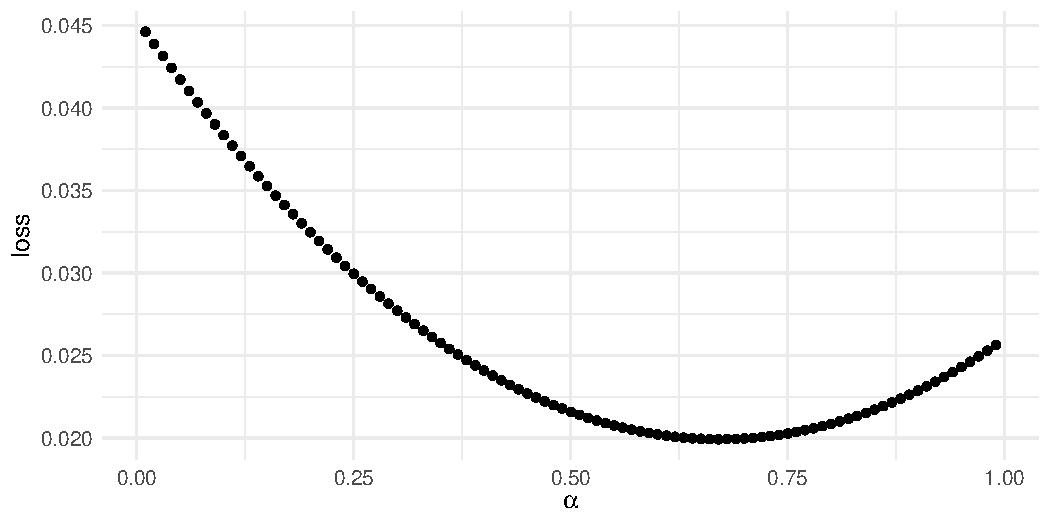
\includegraphics[width=\maxwidth]{figure/cv_benchmark-1} 

}

\caption[Out-of-sample variance estimates from the 5-fold cross-validation]{Out-of-sample variance estimates from the 5-fold cross-validation.}\label{fig:cv_benchmark}
\end{figure}

\end{knitrout}

In Figure \ref{fig:cv_benchmark} the out-of-sample variance, aggregated over folds, is displayed. 
Cross-validation suggests that the optimal value should be $0.67$. 
The analytic method from \citet{bodnar2018estimation} suggests that the optimal value is $0.7926$.
The "correct" value of $\alpha$, as given by the oracle estimator $\hbw_{SH}^\top\bSigma \hbw_{SH}$, is equal to $0.8113$. 
Although none of the methods are spot on, the bona-fide estimator is closer to what the optimal value should be.
Furthermore, changing the number of folds in the code above can give quite different results in the optimal value.
In this example, CV does not seem to be stable when used in conjunction with large dimensional portfolios.
For this specific application, there is value in deriving a bona-fide estimator in terms of the loss and shrinkage estimator.
This approach is used in papers \hyperref[sec:paper3]{3}, \hyperref[sec:paper4]{4} and \hyperref[sec:paper5]{5}.

Shrinking the weights can provide a good estimator in higher dimensions. 
As previously stated, another approach is to shrink the elements of $\bS$.
If the sample covariance matrix is shrunk, then the concentration ratio $c$ can be greater than one.
This is the topic of the last paper of this thesis which is left for the next section where the papers are described in more detail.
%\begin{enumerate}
%	\item Other types of estimators and why they might be better than $\bS$.
%	\item Rotation-invariant estimation - what does it mean (we do not want to target eigenvectors)?
%\end{enumerate}

%%%%%% ------------------------------------------------------------------------
\chapter{Summary of papers}\label{ch:papersummary}
%%%%%% ------------------------------------------------------------------------


The following papers are included in this thesis.
\section{Paper 1 - Sampling distributions of optimal portfolio weights and characteristics in small and large dimensions}\label{sec:paper1}
The paper investigates a fundamental question in MPT. 
What are the actual implications of using the sample covariance matrix $\bS$ and the sample mean $\byb$ instead of the true covariance matrix $\bSigma$ and mean vector $\bmu$?
The paper presents an answer to the question when the returns follow a multivariate normal distribution. 
It contains the distribution for all optimal portfolios on the common form
\begin{equation}\label{eqn:paper1_eq1}
  \bL\hbw_{opt} = \bL\hbw_{GMV} + g(\hR, \hV, \hs)\frac{\bL\hat{\bQ}\byb}{\hs}
\end{equation}
for some matrix $\bL$ of size $k \times p$ where $k<p$.
The joint distribution of all quantities in \eqref{eqn:paper1_eq1} is derived through a stochastic representation. 
The stochastic representation can be used to efficiently simulate from the distribution.
By simulation, quantities such as quantiles or other summary statistics are easily computed.
Furthermore, the high-dimensional asymptotic joint distribution is also derived. 
In a simulation study, the high-dimensional asymptotic distribution is compared to simulated data.
One scenario considers simulations from the stochastic representation, trying to deduce the finite-sample properties of the high-dimensional distribution.
The other scenarios try to investigate what happens when observations deviate from the model.
As expected, the high-dimensional distribution works well under the assumptions and seems to be reasonably robust from deviations of the model.
The GMV and self-financing portfolio are the most robust quantities to deviations from the model.

\section{Paper 2 - Tangency portfolio weights under a skew-normal model in small and large dimensions}\label{sec:paper2}
In this paper, the implications of skewness on the Tangency Portfolio (TP) from Chapter \ref{ch:MPT} is investigated. 
The portfolio is obtained from the quadratic utility function, namely
\begin{equation}
  \min_{\bw} \bw^\top (\bmu -r_f\ones) - \frac{\gamma}{2} \bw^\top \bSigma \bw.
\end{equation}
This paper extends paper 1 as it considers investments in a risk-free asset and use an extension of the multivariate normal model, the CSN model presented in Chapter \ref{ch:estim}. 
The model can include skewness in the asset returns, a trait returns usually exhibit (see e.g., \citet{cont2001empirical}). 
Similarly to paper 1, the distribution of the sample tangency portfolio is derived and the implications the skewness has on the portfolio.
In short, skewness results in a bias present in the portfolio weights. 
An investor will not hold the correct portfolio on average.
Furthermore, the high-dimensional distribution of the sample tangency portfolio is derived.
It can be seen that the skewness disappears asymptotically. 
The high-dimensional distribution is the same as previous research has shown (see, e.g., \citet{karlsson2021statistical}).

\section{Paper 3 - Dynamic shrinkage estimation of the high-dimensional minimum-variance portfolio}\label{sec:paper3}
This paper solves a practical feature when investing in the GMV portfolio: how to rebalance the portfolio at fixed time points. 
If an investor owns a GMV portfolio and waits for a week, month or year the data will likely indicate that another GMV portfolio should be held.
The change can be quite large if $n$ is sufficiently small.
A natural question to ask is how to go from one portfolio to another, e.g., how to rebalance optimally when a new set of data is available. 

In this paper, a dynamic rebalancing scheme for the GMV portfolio is derived. 
The scheme aims to decrease the out-of-sample variance between the holding portfolio, which might be a random GMV portfolio, and the GMV portfolio that is suggested by the current period's data. 
The portfolios are on the following form
\begin{equation}
  \hbw_{SH;n_{i}}=\psi_{i}\hbw_{S;n_i}+ (1-\psi_{i})\hbw_{SH;n_{i-1}},
\end{equation}
where $\hbw_{S;n_i}$, $i=1,2,...,T$, is the traditional sample GMV portfolio using the $i$th sample of size $n_i$ to estimate the GMV portfolio weights in \eqref{eqn:GMV}. 
The initial portfolio, $\hbw_{SH;0}$, can be a random GMV portfolio or a deterministic target portfolio $\bb$.
It is assumed that an investor has specified dates $t_i$, $i=1,2,...,T$ that he/she wants to rebalance his/her GMV portfolio. 
The shrinkage coefficients are then determined through the following optimization problem
$$
\min_{\psi_i} \hbw_{SH;n_{i}}^\top \bSigma \hbw_{SH;n_{i}}.
$$
The problem is similar to the linear shrinkage discussed in Chapter \ref{ch:highdim}.
The portfolio allocation problem is an extension to the work of \citet{bodnar2018estimation} and uses the flexible location and scale model in \eqref{eqn:location_scale_model}.

The portfolio is shown to produce great results in an extensive simulation study.
It also provides a better estimator for the volatility in comparison to the traditional sample GMV as well as the GMV portfolio using \citet{lw20} nonlinear shrinkage estimator for the sample covariance matrix.
There are also many other benefits of using the portfolio strategy.
Transitions from one portfolio to the next costs money, which will diminish the return and profit that can be made.
Furthermore, it is not always possible to go from one portfolio to the next in a day or even a month.
The traditional GMV portfolio might suggest that an institution should first own a large long position and the next month a large short position.
Depending on the size of the institution and the portfolio, the size of these positional changes might be illegal. 
It can be deemed market influencing or just outright impossible to sell that many assets.
The rebalancing scheme provides a solution to these problems.

\section{Paper 4 - Is the empirical out-of-sample variance an informative risk measure for high-dimensional portfolios?}\label{sec:paper4}
Any empirical application using the GMV portfolio is bound to include the volatility or variance as a performance measure. 
However, the empirical out-of-sample variance is not consistent.
Is the empirical out-of-sample variance for a shrunk portfolio a consistent estimator of the variance? 
Furthermore, is it a good option to use or are there perhaps better options to use as performance measures? 
This paper investigates two different metrics of evaluation that are common to the GMV portfolio, the out-of-sample variance and the relative out-of-sample loss.

This paper also considers the location and scale model from \eqref{eqn:location_scale_model} and three different GMV portfolios. 
The first portfolio is the traditional GMV portfolio from \eqref{eqn:GMV}, the second is the portfolio from \citet{bodnar2018estimation} and the last is the linear shrinkage portfolio from \citet{frahm2010}.
The properties of the out-of-sample variance, relative loss and their empirical counterparts are derived for the three different portfolios. 
It is done under different assumptions on the parameters of the model.
Most notably, there is a natural ordering to the different out-of-sample losses.
The empirical out-of-sample loss is smallest for \citet{bodnar2018estimation}, second to smallest is \citet{frahm2010} and the largest is the traditional sample GMV portfolio.
Furthermore, the empirical out-of-sample variance for the different portfolios are presented.
The assumptions that are necessary for convergence of the empirical out-of-sample variance are quite different from those used for the empirical out-of-sample loss.
The assumptions necessary for convergence of the empirical out-of-sample variance are deemed stronger than the empirical out-of-sample loss.
The theoretical findings are investigated in a simulation study and an empirical application which validate the ordering even when the model assumptions are violated.

\section{Paper 5 - Two is better than one: Regularized shrinkage of large
minimum variance portfolios}\label{sec:paper5}
The methods of this thesis most often use the sample covariance matrix $\bS$.
They deal with the fact that the sample covariance matrix is a noisy estimator for the portfolio weights by linear shrinkage on the weights themselves.
The estimator can only cover $c<1$.
This paper introduces a Thikonov regularization on the portfolio weights together with the linear shrinkage from prior papers. 
It results in a ridge type estimator for the sample covariance matrix together with the linear shrinkage on the portfolio weights.
There are two shrinkage types, one which put constraints on the sample covariance matrix and one which controls the weights.
This approach enables the method to cover the case where $c>1$ as well as let an investor input his/hers beliefs in the portfolio allocation problem.
The portfolio looks like
$$
\hbw_{SH} = \psi \frac{\left(\bS + \eta \bI_p \right)^{-1}\ones_p}{\ones_p^\top\left(\bS + \eta \bI_p \right)^{-1}\ones_p} + (1-\psi)\bb.
$$
The natural loss for estimating $\psi$ and $\eta$ is the out-of-sample variance.
It turns out it is not possible to construct a closed-form oracle estimator for the shrinkage parameters.
However, there is a possibility to construct an oracle loss function, for which a bona-fide estimator can be derived.
The bona-fide loss is proved to be a consistent estimator of the oracle loss.

The model is seen to perform on-par with the nonlinear shrinkage of \citet{lw20} in all simulations.
Further, the method consistently beats the \citet{lw20} method in an extensive empirical analysis.
The regularized shrinkage approach provides the best out-of-sample variance for five out of six different configurations.
Furthermore, the method also increases the performance of several other portfolio metrics.

%\section*{Paper 6 - The capital market line, tangency portfolio and the effect of Tikhonov regularization in higher dimensions}\label{sec:paper6}

\section{Other research results}\label{sec:other_results}

Paper 3 is accompanied by the DOSPortfolio R-package (see, \citet{DOSPortfolio}), available on CRAN. 
The readers of this thesis are free, or rather encouraged(!), to install it with \hlkwd{install.packages}\hlstd{(}\hlstr{"DOSPortfolio"}\hlstd{)}. 
The package provides a simple interface for the methods implemented in the paper. 
In \ref{DOSportfolio} a short example on how to construct the dynamic portfolio weights using the package is displayed. 
The package is the first iteration of possibly many more portfolios which can be constructed in a similar fashion.
\begin{knitrout}\small
\definecolor{shadecolor}{rgb}{1, 1, 1}\color{fgcolor}\begin{kframe}
\captionof{chunk}{R-code which showcase the use of the DOSPortfolio package.}\label{DOSportfolio}\begin{alltt}
\hlkwd{library}\hlstd{(DOSPortfolio)}
\hlstd{df} \hlkwb{<-} \hlkwd{read_csv}\hlstd{(}\hlstr{"../data/returns.csv"}\hlstd{)}
\hlstd{p} \hlkwb{<-} \hlnum{350}\hlstd{; n} \hlkwb{<-} \hlnum{400}
\hlcom{# Sample p assets}
\hlkwd{set.seed}\hlstd{(}\hlnum{1234}\hlstd{)}
\hlstd{asset_cols} \hlkwb{<-} \hlkwd{sample}\hlstd{(}\hlnum{2}\hlopt{:}\hlkwd{ncol}\hlstd{(df),} \hlkwc{size} \hlstd{= p)}
\hlcom{# specify reallocation points, daily in this case}
\hlstd{reallocation_points} \hlkwb{<-} \hlkwd{seq}\hlstd{(n,} \hlkwd{nrow}\hlstd{(df),} \hlkwc{by}\hlstd{=n)}
\hlcom{# estimate portfolio weights}
\hlstd{dos_weights} \hlkwb{<-} \hlstd{df} \hlopt
  \hlkwd{select}\hlstd{(}\hlkwd{all_of}\hlstd{(asset_cols),} \hlopt{-}\hlstd{date)} \hlopt
  \hlkwd{DOSPortfolio}\hlstd{(}\hlkwc{reallocation_points} \hlstd{= reallocation_points,}
               \hlkwc{target_portfolio} \hlstd{=} \hlkwd{rep}\hlstd{(}\hlnum{1}\hlstd{,} \hlkwd{ncol}\hlstd{(.))}\hlopt{/}\hlkwd{ncol}\hlstd{(.),}
               \hlkwc{shrinkage_type} \hlstd{=} \hlstr{"overlapping"}\hlstd{)}
\end{alltt}
\end{kframe}
\end{knitrout}
Furthermore, the following papers were co-authored throughout the writing of this thesis: \cite{bodnar2020quantile}, \cite{bodnar2021bayesian}  and \cite{bodnar2021quantile}.
The first presents an analytic derivation of the MPT framework in the Bayesian setting. 
It specifically investigates how quantiles of optimal portfolios can be constructed and the effects of estimation uncertainty in these. 
This is especially important since the regulations in place demands that quantile-based risk measures are reported (see \citet{basel4}).
The second paper provides a continuation on the first. 
The idea is to model the belief of an investor in a prior distribution. 
The method then aims to construct the prior distribution to capture what the likelihood cannot. 
It imposes a prior distribution which adapts to the recent observations when the market is turbulent. 
The algorithm is seen to work well when markets are turbulent.
The third paper also considers quantile-based portfolios. 
The paper does so in a general framework, not necessarily the same framework as MPT where the first two moments of the return distribution are used.



%%%%%% ------------------------------------------------------------------------
\chapter{Future research}\label{ch:future}
%%%%%% ------------------------------------------------------------------------


%% What the methods assume
% independence, validate through simulations though there is no general guarantee that it works.
% Sigma having bounded support, especially paper 5.
The methods of this thesis all rely on one concept, the observations from the joint asset return distribution are iid.
Paper \hyperref[sec:paper2]{2} use a special case of the CSN model.
This is the only model which has the potential to incorporate more developed time series dynamics in the data.
The methods and theory from papers \hyperref[sec:paper1]{1} and \hyperref[sec:paper2]{2} cannot work under the more general data generating process.
The models used in papers \hyperref[sec:paper3]{3} through \hyperref[sec:paper5]{5} also assume iid observations.
In these papers, the methods are tested through simulations.
The simulation studies show that the methods are robust to deviations from the iid assumption.
However, this thesis does not provide an explanation to what effect deviations from the assumption has on the portfolio estimates.
Deriving the effects of the time dependency could help an investor understand the results of their investment strategy and portfolio.

The next assumption used in this thesis is that $\bSigma$ were to have bounded eigenvalues.
A common model for pricing assets is arbitrage pricing theory and factor models. 
One of these models are used in the simulation study of papers \hyperref[sec:paper3]{3} through \hyperref[sec:paper5]{5}, the Capital Asset Pricing Model (CAPM).
There are many motivations for using it (see, e.g., \citet{ross2013arbitrage}), which will not be discussed here.
By imposing structure in the model, it reduces the number of parameters that needs to be estimated.
It omits some parts of the problems that the methods of this thesis are faced with.
However, \citet{fan2013large} showed in such a model, the largest eigenvalue of the sample covariance matrix is of order $p$.
It does not have bounded spectral norm.
This can sometimes be circumvented but not in others.
The methods in Paper \hyperref[sec:paper5]{5} have to assume that the spectral norm of $\bSigma$ is bounded, otherwise some quantities in the proofs diverge.
Removing the assumption could provide more theoretical justification for the method though the simulations study from Paper \hyperref[sec:paper5]{5} indicates that it is robust against deviations from this assumption.

There are many possible extensions and future projects to the thesis at hand.
Estimation uncertainty is the primary motivation for this thesis.
Bayesian statistics provide a straightforward way to integrate that. 
However, it demands indepth knowledge of Markov Chain Monte Carlo and also how to construct good prior distributions.
Neither are easy tasks.
Another approach of incorporating estimation uncertainty is robust optimization.
In the MPT setting, robust optimization tries to incorporate the estimation uncertainty into the portfolio allocation problem itself.
Are there connections to be made and especially with empirical Bayes?

Paper \hyperref[sec:paper3]{3} assumes that the rebalancing points are fixed.
This assumption can be limiting for some investors.
Can those be exchanged for stopping times, incorporated in the decision process and the portfolio allocation problem?

Many Multivariate GARCH models can be formulated as the following BEKK model (see, e.g., \citet{engle1995multivariate})
\begin{equation}\label{eqn:BEKK}
  \bH_t = \bC \bC^\top + \sum_{k=1}^K \bA_k \boldsymbol{\epsilon}_{t-1}\boldsymbol{\epsilon}_{t-1}^\top \bA_k^\top + \sum_{k=1}^K \bG_k \bH_{t-1}\bG_k^\top,
\end{equation}
where $\bH_i$ is a sequence of conditional covariance matrices, $\boldsymbol{\epsilon}_t | \mathcal{F}_{t-1} \sim N_p(\mathbf{0}, \bH_t)$ and the matrices $\bC, \bA_i$ and $\bG_i$ are of appropriate dimensions.
These are usually very hard to fit and use for portfolio allocations. 
The first issue is due to the number of parameters in the model.
There are a number of parametrisations but if all matrices are symmetric then there are $(K+1/2)p(p+1)$ parameters to estimate. 
Building a portfolio of size 10 with $K=1$ implies that $165$ parameters need to be estimated.
Furthermore, although the constraints should enforce forecasts which are positive definite it is not necessarily true that they will be numerically invertible.
It can provide forecasts which are very close to singular.
The first issue can be solved if one can formulate the models as Recurrent Neural Networks and use deep-learning libraries Torch or Tensorflow to fit the models. 
These are tailored to solve the problem of fitting very large models.
Recent large Natural Language Processing models have \textit{billions} of parameters (see, e.g., \citet{brown2020language}). 
The second issue can then possibly be solved by placing BEKK models in this framework.
Positive definite forecasts could then be enforced by developing new layers to the network. 
Furthermore, it would also be easier to integrate different sources of information, such as sentiment, in the models.

\chapter{Svensk sammanfattning}
Portföljer med finansiella instrument och diversifiering går oftast hand i hand.
Diversifiering är ett, om inte det bästa, verktyget för att minska risken i en portfölj.
Om en av investeringarna skulle gå dåligt spelar det ingen roll för den utgör en sådan liten del av portföljen.
Modern Portföljteori (MPT) är ett ramverk för att konstruera diversifierade portföljer.
Ett hinder är dock att MPT använder okända parametrar.
Dessa okända parametrar är de två första momenten av tillgångarnas avkastningsfördelning.
När dessa ersätts av skattare introduceras estimerings-osäkerhet.
Om en investerare inte förstår osäkerheten finns det en risk att den dominerar alla resultat som portföljen, eller strategin, skulle kunna påvisa.
Det finns inget sätt att avgöra om strategin fungerar eller inte.

Denna avhandling innehåller fem artiklar.
De innehåller resultat som kan hjälpa en investerare att hantera skattningsosäkerhet i oändliga portföljer samt, i vissa fall, beskriva portföljernas fördelning för ett ändligt stickprov.
Dessa resultat gör det lättare för investerare att förstå investeringsprocessen och de empiriska resultat som kan observeras i praktiken.

Artikel I utforskar alla portföljer i MPT-ramverket.
I artikeln härleds alla optimala portföljers empiriska fördelning, det vill säga när skattare används istället för de sanna parametrarna.
Det inkluderar fördelningen för vikterna samt den avkastning, varians och andra mått som karateriserar dessa portföljer.
Därefter härleds den asymptotiska fördelningen för alla mått samt vikter i stora dimensioner.
Denna fördelning kan ses som ett fall då en investerare diversifierar oändligt mycket i MPT-ramverket samt har oändligt mycket data gällande de tillgångar han/hon investerar i.
En simuleringsstudie visar att den asymptotiska fördelningen utgör en god approximation av fördelningen för ändliga stickprov, givet att modelantagandet håller.

Artikel II fortsätter vidare på artikel I.
I denna artikel undersöks portföljen från det kvadratiskt nytto-optimeringsproblem med en riskfri tillgång. 
En riskfri tillgång kan exempelvis vara ett räntebärande konto.
Denna portfölj är också känd som den tangerande portföljen.
I artikeln härleds den empiriska fördelningen för portföljvikterna fast med en generalisering av modellen från artikel I.
Fördelningen för tillgångarna antas vara skev-normal.
Resultaten visar att skevhet gör att de empiriska vikterna i portföljen är i genomsnitt fel.
Detta sker i genomsnitt för ändliga stickprov men den empiriska portföljen skattar rätt objekt i stora dimensioner. 

Artikel III ger en lösning på problemet att äga en portfölj för att sedan gå över till en annan.
I artikeln utvecklas en metod som omfördelar portföljen på givna tidpunkter.
Den gör detta genom att minimera den framtida variansen för Minsta Varians (GMV) portföljen, givet att en investeraren redan äger en portfölj.
Portföljen som ägs i denna stund kan vara deterministisk eller en skattad GMV-portfölj.
En omfattande simuleringsstudie visar att denna metod kan uppnå goda resultat i termer av att skatta den relativa förlusten.
Den relativa förlusten är en enkel utveckling av portföljvariansen.
Metoden utvärderas därefter med hjälp av marknadsdata.
Den lyckas bäst i att ge minsta framtida varians samt ge de minsta förändringarna i portföljvikterna bland de olika metoderna i jämförelsegruppen.
Metoden har implementerats i ett R-paket som heter DOSPortfolio och finns tillgängligt på CRAN. 

Artikel IV härleder olika egenskaper för två olika prestandamått av tre olika skattare för GMV-portföljer.
Prestandamåtten är den framtida variansen samt den framtida relativa förlusten för GMV-portföljerna.
Det tidigare nämnda prestandamåttet används närpå alltid för att utvärdera GMV-portföljer med empirisk data.
Resultaten visar att den relativa förlusten inte behöver lika strikta antaganden för att konvergera i stora dimensioner.
Detta mått kan därför täcka flera modeller till skillnad från variansen.
Prestandamåtten används sedan för att bestämma en ordning på de olika portföljerna.
Dessa resultat verifieras i en simuleringsstudie samt med empirisk data. 

Artikel V utvidgar en av GMV-portföljerna från artiklarna III och IV.
I den här artikeln introduseras en Thikonov-regularisering på portföljvikterna vilket resulterar i en Ridge-liknande skattare för den empiriska kovariansmatrisen.
Detta kombineras sedan med den linjära shrinkage-metoden från artiklarna III och IV.
Denna portfölj undersöks sedan i en omfattande simuleringsstudie och dess prestanda studeras med empirisk data.
Simuleringsstudien visar att metoden är jämförbar med ett flertal metoder.
Den empiriska studien visar att metoden som utvecklas ger lägre skattningar av framtida varians än ett flertal referensportföljer samt att den visar bra prestanda gällande portföljvikterna.

\backmatterSU

\printbibliography[keyword={ref_list}]
%%%%%%%%%%%%%%%%%%%%%%%%%%%%%%%%%%%%%%%%%%
% Insert papers here
%%%%%%%%%%%%%%%%%%%%%%%%%%%%%%%%%%%%%%%%%%
\part{Papers}
\end{document}
